%!TEX root = ../thesis.tex
%*******************************************************************************
%****************************** Second Chapter *********************************
%*******************************************************************************

\chapter{Clustering single cell RNAseq by genotypes in mixed samples.}

\ifpdf
    \graphicspath{{Chapter2/Figs/Raster/}{Chapter2/Figs/PDF/}{Chapter2/Figs/}}
\else
    \graphicspath{{Chapter2/Figs/Vector/}{Chapter2/Figs/}}
\fi



%********************************** %First Section  **************************************
\section{Background}
\par{
Cells are a natural discrete building block of biology. And tissues are almost always complex arrangements of multiple different cell types. Bulk RNAseq is a blunt 
instrument measuring the average RNA content of many cells in a tissue. 
Advances in methods for the preparation of samples containing minuscule amounts of nucleic acids have made it possible to study the transcriptional state of single cells \cite{first_singlecell}.
Single cell RNAseq (scRNAseq) is the process of measuring the transcriptional profile of each cell individually usually by physically separating cells into and delivering distinct barcode sequences to templates generated from the mRNA of each cell \cite{smartseq2}.
Further advances in nanodroplet and nanowell technologies have made it possible to apply scRNAseq to thousands of cells simultaneously \cite{dropseq}\cite{10xsinglecell}\cite{seqwell} instead of the plate based strategies which usually were applied to hundreds of cells at a time \cite{smartseq2}. 
}





\par{
Many samples contain cells of mixed genotypes including those of single celled organisms such as mixed strain malaria infections, 
the gut microbiome, and environmental samples as well 
as intrinsically mixed samples such as maternal/fetal, transplant patient, or tumor samples and intentionally multiplexed samples.
Additionally, mixing cells from multiple individuals into a single experiment has become a popular experimental design because it makes the data more comparable between individuals, reduces costs, and can improve doublet detection. 
 In order to properly 
analyze this data we must first identify each cell's genotype of origin. Some tools and methods exist for this purpose \cite{demuxlet} \cite{cellhashing} \cite{scsplit} 
but each of them contain some downside such as the need for prior knowledge of the genotypes or experimentally attaching a sample barcode before mixing cells, and all of them 
contain several error modes arising from the lack of modeling the ambient RNA in the system. Ambient RNA in single-cell RNAseq (also known as soup) is a recently described 
phenomenon in which RNA molecules from cells that have lysed before cell partitioning are included in partitions with cells from which they did not originate \cite{soupx}. This adds noise to both the transcriptional profiles of the scRNAseq experiment, but also the genotype analysis and demultiplexing of mixed genotype samples. 
In these demultiplexing systems, not modeling the ambient RNA makes many cells appear to be doublets and makes many homozygous variant sites appear to be 
heterozygous. 
}

\par{
In this chapter, I present souporcell, a tool containing a collection of algorithms to support mixed genotype scRNAseq experiments\cite{souporcell}. 
To use the genetic variants measured in the RNAseq reads to assign cells to their donor of origin, first we must describe a strategy for calling reliable variants in scRNAseq data (figure \ref{fig:souporcell}a,b) and assigning allele counts to cell barcodes (see figure \ref{fig:souporcell}c). We then describe the core algorithm of souporcell, that of clustering cells by their genetic variants in the face of the sparse measurements of expressed alleles by each cell (figure \ref{fig:souporcell}d). Next we describe the algorithm used for determining which barcodes represent multiple cells instead of a single cell (figure \ref{fig:souporcell}e). And finally we describe a statistical model and coinference of the cluster genotypes and amount of ambient RNA there is in the experiment (figure \ref{fig:souporcell}f). 
}


\begin{figure}[th!]


\begin{centering}
\caption{souporcell overview}\label{fig:souporcell}

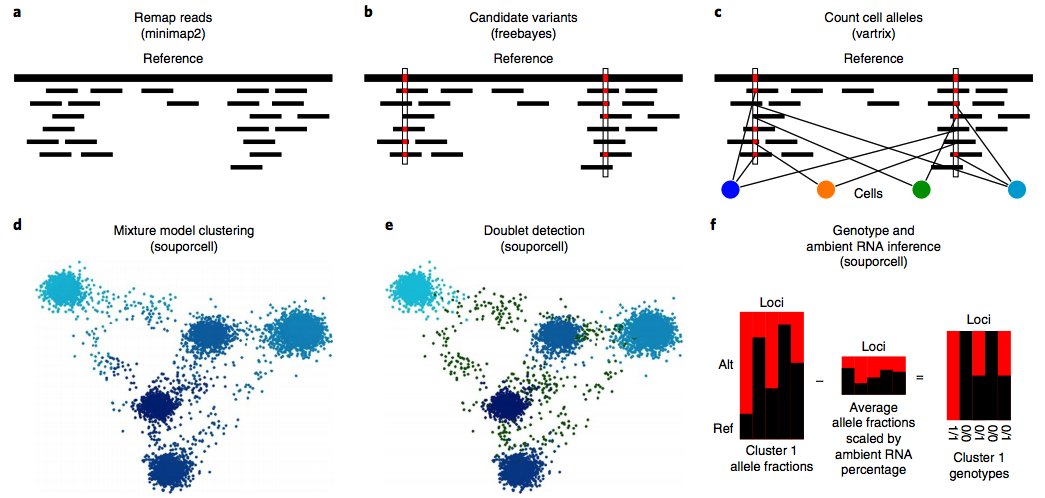
\includegraphics[width=\textwidth]{main.png} 

\par{\textbf{a)} We first remap the reads using minimap2, retaining the cell and UMI barcode for downstream use. b,c, We then call
candidate variants using freebayes \textbf{b} and count the allele support for each cell using vartrix \textbf{c}. \textbf{d)} Using the cell allele support counts, we cluster the cells with sparse mixture model clustering (Methods). \textbf{e,f)} Given the cluster allele counts, we categorize cells as doublets (\textbf{e}) or singletons and,
excluding doublets, we infer both the fraction of ambient RNA and the genotypes of each cluster (\textbf{f}; see example for one cluster). Alt, alternate allele;
ref, reference allele.}
\end{centering}
\end{figure}
\par{
We then demonstrate and benchmark souporcell against a dataset which was mixed in silico and thus we retain full knowledge of the ground truth of which barcodes came from which individual, which barcodes represent cross-genotype doublets, and how much ambient RNA was simulated (see figure \ref{figure:synthetic}). To show that this dataset is a realistic example, we then show the same results on an experimental mixture of cells from those same individuals(shown in figure \ref{figure:real}).
}
\par{
We compare our method to demuxlet, the previous gold standard method that requires genotype information a priori, as well as two new tools that, like souporcell, do not require prior genetic information\cite{vireo}\cite{scsplit} on the in silico mixture with various aspects of the data (doublet rate, ambient RNA amount, minority cluster size) swept and evaluate clustering, doublet detection, and ambient RNA detection across a wide range of data charactaristics. We sought to test souporcell on more challenging cases and chose that of highly related individuals by demultiplexing maternal-fetal placental and decidual experiments. We also test on mixtures of the malaria parasite, \textit{Plasmodium falciparum}, which is challenging due to the cells having much lower expression levels than the human cells previously tested.
}
\par{
We show that souporcell not only outperforms the competing methods, but also surpasses the previous gold standard, demuxlet, on both cell assignment and doublet accuracy. Furthermore, souporcell explicitly models and estimates the amount of ambient RNA in the experiment, which is a major confounder of scRNAseq analysis with regard to both expression and genotype. Although a tool for ambient RNA quantification exists\cite{soupx}, it requires prior knowledge in the form of one or more well expressed genes known to not be expressed in a particular cell type. Souporcell is freely available under the MIT open source license at https://github.com/wheaton5/souporcell.
}


\section{Methods} %Section - 1.1 
\subsection{Variant calling on scRNAseq data}
In order to use the genetic variants in the scRNAseq reads to assign cells to individuals, we must first call the variants accurately and assign which alleles were expressed by which cells. Little work has been done on identifying genetic variants in bulk RNAseq \cite{RNAvariant} let alone scRNAseq \cite{vartrix}\cite{cellsnp}. 



\subsubsection{Remapping}
\par{
Currently, the most popular software for the initial analysis of droplet based scRNAseq data to go from the reads to the mRNA expression matrix is cellranger \cite{10xsinglecell}. In the cellranger pipeline, the reads are first mapped to a reference genome. RNA mapping and DNA mapping software differ due to the intended downstream uses. With DNA mapping, accurate variant calling is one of the primary applications and thus much work has been put into providing accurate mapping quality scores and base level alignments making single nucleotide polymorphisms (SNPs) and short insertions and deletions (indels) easy to call accurately versus the reference genome used \cite{bwa}\cite{minimap2}\cite{bowtie}\cite{freebayes}\cite{gatk}. The mapping and alignment operations are relatively computationally costly if accurate variant calling is not one of the desired downstream uses. RNA mapping applications are usually primarily concerned with just counts of reads per gene and sometimes differential RNA splicing. Thus, the RNA community has developed software some of which are faster but do not provide base level alignments \cite{kallisto}\cite{salmon} and others that allow for gapped alignments caused by the introns being spliced out \cite{bowtie2}\cite{STAR}\cite{hisat}\cite{tophat}. But in optimizing for the downstream applications of transcript counting and differential splicing, genetic variant calling accuracy can suffer. In cellranger, the mapping component is done with the STAR aligner \cite{STAR} which, while sufficient for the purpose 
of counting gene expression, produces artifacts in the alignments that produce many false positive variants. 
}
\par{
One such source of false positives is the 
soft clipping penalty which is not a parameter exposed to the user in the STAR software. It is often the case in WGS and even more so in RNAseq that the starts and ends of
reads can be less reliable than the rest of the read. In addition to this, base level alignments toward the ends of reads can be error prone because there is not a sufficient amount of sequence remaining for the ``correct" alignment to be the optimal alignment according to the alignment score. For example, an alignment may prefer to take several single base mismatch penalties rather than a single true indel penalty. This tradeoff is more likely to happen towards the end of the read when there are fewer bases remaining to align (see figure \ref{fig:softclipping}b). Because of this, mappers built for variant calling such as BWA \cite{bwa} and minimap2 \cite{minimap2} have 
a relatively small one-time penalty for soft clipping any number of bases from the end of an alignment \cite{variantartifacts}. The STAR alignment soft clipping penalty is such that, in 
comparison with other aligners, it can create many false positive variant calls produced entirely by bases at the ends of reads (see figure \ref{fig:softclipping}b). Another source of 
small variant errors caused by the STAR alignments is that the default indel penalty relative to the mismatch penalty is much higher than that of 
variant calling ready aligners. These penalties will, for example, prefer inducing 10 single base mismatches rather than a single 12 base indel. Further, it will make the same error for all of the reads spanning the indel and these bases but not those spanning those bases but not spanning the indel causing those mismatches to potentially appear to be heterozygous genetic variants. 
}


\begin{figure}[htbp!]


\begin{centering}
\caption{Star alignments' indel and soft clipping problems}\label{fig:softclipping}

%\begin{subfigure}{0.75\textwidth}
\sidesubfloat[]{
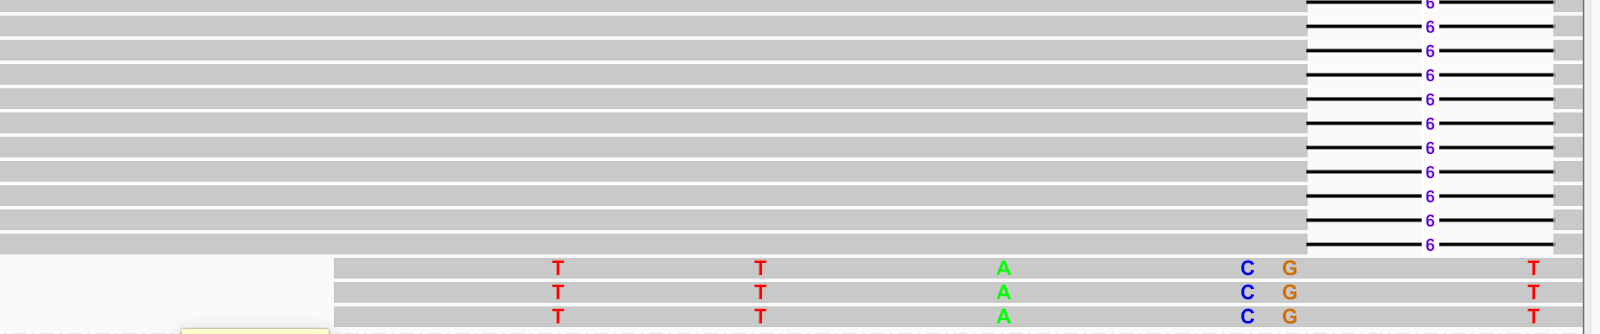
\includegraphics[width=0.75\textwidth, valign=t]{star_indel_issue.png} \label{fig:a}
}
%\end{subfigure}

%\begin{subfigure}[t]{0.75\textwidth}
\sidesubfloat[]{
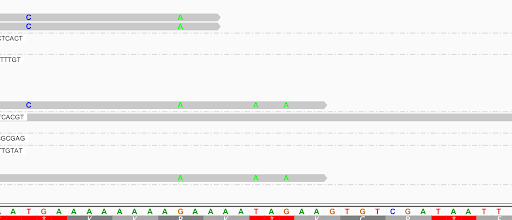
\includegraphics[width=0.75\textwidth, valign=t]{softclipping.png} \label{fig:b}
}
%\end{subfigure}

\textbf{a)} Reads that span more bases find a six base indel, but ones that span fewer bases incur many erroneous single base mismatches without soft clipping. Minimap2 finds this indel in all of the shown reads and soft clips some others with even later start positions. \textbf{b)} In the second example, the reads have an adenosine homopolymer and partially match this section of the reference. Minimap2 softclips these reads. 
\end{centering}
\end{figure}
\par{
The indel penalty is exposed as a parameter to the user, but with the default parameters (and thus with the output of cellranger) these errors exist. 
And finally, the last source of errors these alignments induce are due to the leniency of spliced alignments which STAR has. With its default parameters including 
a max intron length of 200kb, STAR will often include erroneous and statistically spurious spliced alignments of reads that otherwise don't align well. This creates alignments 
which match for some statistically significant portion in one location and then are spliced to other loci often for as low as an eight base segment which should occur by 
random chance alone. Due to the nature of mapping qualities being assigned to the whole alignment and not each segment of the alignment, these sections are often denoted as 
having a high mapping quality when in fact the matches should occur by chance. If there is actually an alternative allele in one of these regions to which some reads have 
spurious matches, those reads, and thus those cells, appear to support the reference allele. These alignments provide one further technical 
issue, which is that they dramatically slow down the pileup and fetch commands in samtools \cite{samtools} which are necessary for variant calling. 
}
\par{
For these reasons we first remap the data with either BWA, minimap2, or hisat2. We have found good results when remapping with minimap2 with a combination 
of long read splice parameters and short read parameters. Specifically, the parameters for which all analysis is done in this thesis are the following: 
minimap2 -ax splice -t 8 -G50k -k 21 -w 11 --sr -A2 -B8 -O12,32 -E2,1 -r200 -p.5 -N20 -f1000,5000 -n2 -m20 -s40 -g2000 -2K50m --secondary=no. We then perform 
deduplication by removing reads with the same unique molecular identifier (UMI) barcode, cell barcode, and have the same start and stop position.
}


\subsubsection{Variant Candidate Calling}
\par{
Once we have an accurately mapped alignment file, we must then proceed to variant calling. We assessed two strategies for calling variants on scRNAseq and assigning alleles to cell barcodes. We first treated 
the sample as a population of cells and called variants with a population variant caller \cite{freebayes} \cite{gatk} \cite{samtools}. With this approach we assigned each cell barcode to its own read group in the input bam and the variant caller produces a population VCF with genotype calls for each cell for each locus.
We also assessed treating the sample as an unknown mixture of haplotypes, called variants on that unknown mixture, and then for each read (and thus its cell barcode) decide whether it supports the reference allele or alternative allele which can be done with the tool vartrix\cite{vartrix}. Our analysis suggests these two strategies perform very similarly. 
}
\subsubsection{Cell allele assignment}
\par{
Because the latter strategy is much more computationally efficient, all further analysis is done with freebayes with parameters --pooled-continuous -iXu -C 2 -q 20 -n 3 -E 1 -m 30 --min-coverage 6 and vartrix with parameters  --umi --mapq 30 --scoring-method coverage which will return a sparse matrix market format indicating how many of the reference allele or alternative allele each cell barcode expressed for each variant locus. Vartrix works by aligning each read to the reference sequence as well as the variant sequence to determine which one it supports. Doing this rather than simply inspecting the base level alignment improves reference bias and alignment end effects. For example, when assessing if a read supports an insertion of an A in a homopolymer of adenosines and the read does not extend past that homopolymer, the read will align without the insertion even if it came from the haplotype with the insertion. Aligning to both underlying sequences will produce the same alignment score and we can say that it is ambiguous which allele the read represents.
}
\subsubsection{Validation: Genome in a Bottle}
\par{
We validated our variant calling accuracy by obtaining from 10x Genomics an scRNAseq dataset run on cells from the Genome in a Bottle (GIAB) consortium individual NA12878 cell line for which there is high quality ground truth variant calls available \cite{giab}. As the scRNAseq data will only cover a subset of genes and because this dataset was relatively low coverage, I will primarily focus on false positive rate and not sensitivity. Much of this analysis was done by Yichen Wang as part of a rotation project in our lab. Initially we found a false positive rate of 35.6\%, dramatically higher than the 1-2\% you would have with reasonable coverage whole genome DNA sequencing.
}


\subsubsection{RNA editing}
\par{
We sought to determine the causes of the remaining false positives so identified the false positive SNPs called on the NA12878 scRNAseq data in high confidence regions as defined by the GiaB resource and found that most (80.8\%) of them are purine-to-purine or pyrimidine-to-pyrimidine transitions when we considered the reference and observations. A-to-G and T-to-C transitions happened in much higher frequency than the remaining, making up 59.5\% of
total false positive sites (see table \ref{table:rnaediting}). Calling variants from bulk RNA sequencing data also
displayed a similar pattern, but using whole exome sequencing data did not, linking the
excessive purine-to-purine and pyrimidine-to-pyrimidine transition specifically to RNA seq. We hypothesized that this could be due to RNA editing. The most common RNA editing event is the
deamination of adenosine to inosine on pre-mRNA \cite{atoi}. Inosine is then read as guanosine by
reverse transcriptase, resulting in a T-to-C event in the cDNA, which can explain A-to-G and T-to-C SNPs in variant calling. Visualization in the Integrative Genomics Viewer \cite{IGV} validated the
existence both reads with the false positive allele and reference allele in SNP loci. Moreover, we observed
that the reads that had the same UMI contained the same allele, but not the reads that had
the same cell barcode. This further supported the hypothesis of RNA editing, because the the reverse transcriptase reading inosine as guanine would be consistent for PCR duplicates of the cDNA, but
not necessary for all reads in one cell. And if these were due to sequencing errors, they would not be consistent across all PCR duplicates. To test the hypothesis of RNA editing, we found an RNA editing database (REDIportal\cite{rnaediting}: http://srv00.recas.ba.infn.it/atlas/) and removed the known A-to-I editing sites in our vcf files.
Filtering out RNA editing sites considerably reduced the amount of false positive variants (from
2884 to 1937) and kept most true positive variants (from 8093 to 8073), leading to a reduction
in false positive rate from 35.6\% to 24.0\%. We also discovered that remapping with hisat2
could further reduce false positive rate and improve sensitivity (9540 true positive loci ,1065
false positive loci, false positive rate 11.1\%). However, this work was done after the souporcell paper was published, so the results in this thesis are done with the minimap2 alignments as previously stated.
}

\begin{table}[htb]

\begin{centering}
\caption{RNA editing as a source of false positive variant calls}\label{table:rnaediting}
\sidesubfloat[]{
\begin{tabular}[htb]{|c|c|c|c|c|}\hline

\backslashbox{ref}{obs}&A&T&C&G \\\hline

A & 0 & 54 & 69 & 867 \\\hline
T & 55 & 0 & 849 & 80 \\\hline
C & 77 & 289 & 0 & 75 \\\hline
G & 326 & 68 & 70 & 0 \\\hline
\end{tabular}\label{fig:a}}
\hfil
\sidesubfloat[]{
\begin{tabular}[htb]{|c|c|c|c|c|}\hline

\backslashbox{ref}{obs}&A&T&C&G \\\hline

A & 0 & 54 & 69 & 395 \\\hline
T & 55 & 0 & 376 & 80 \\\hline
C & 77 & 289 & 0 & 75 \\\hline
G & 326 & 68 & 70 & 0 \\\hline
\end{tabular}\label{fig:b}}
\end{centering}
\begin{centering}

\par{\textbf{a)} False positives are primarily purine to purine and pyrimidine to pyrimidine with a notable increase in A->G and T->C caused by the RNA editing adenosine to inosine. The inosine base is then read as a guanine by the reverse transcriptase. \textbf{b)} shows the false positive profile after filtering known RNA editing sites.}
\end{centering}


\end{table}



\subsection{Sparse mixture model clustering}
\par{
In order to introduce this method, we must first motivate it with a description of the data type and its particular difficulties with respect to clustering by genotypes. Each cell barcode has reads from its transcription profile sampled very sparsely. In table \ref{table:scdatatable} I show some basic statistics about two datasets --- one with a mixture of six strains of the malaria parasite \textit{Plasmodium falciparum} which is a unicellular haploid parasitic organism and the sample contains cells coming from all cell types found in the life cycle in the human blood stage. And the other data set is a mixture 
of five human individuals from the human induced pluripotent stem cell project. We use a filter 
requiring at least four cells supporting each allele otherwise the variant is unlikely to be of almost any use in discriminating between different genotypes in this mixture. 
As you can see, the number of cells expressing any given locus is far fewer than the total number of cells and the number of variants with a given number of cells expressing that variant drops off dramatically as cells expressing a given locus increases. It is also evident that while the human data contains more discriminating variants per cell, they are spread over many more total variants thus making the overlap between any two cells very low.
}

\begin{table}[h!]
\caption{Single cell data statistics}
\label{table:scdatatable}
\begin{center}
\begin{tabular}{ | l | l | l | } 
 \hline
  & malaria & human replicate 1 \\ 
  \hline
  number of cells & 2608 & 4925  \\
 \hline
  median UMI per cell & 995 & 25155  \\ 
 \hline
 total variants & 39487 & 194079 \\
 \hline
 median cells per variant & 24 & 18 \\
 \hline
 median variants per cell & 667 & 2642  \\ 
 \hline
 total discriminating variants & 16783 & 77878 \\
  \hline
 median discriminating variant per cell & 512 & 2147 \\
 \hline
 median cells per discriminating variants & 55 & 38 \\
 \hline
 median genes per cell & 571 & 4812 \\
 \hline
 
\end{tabular}
\end{center}
\end{table}

\begin{figure}[th!]
\caption{Single cell sparsity}
\label{figure:scdatafigure}
\begin{centering}
%\begin{subfigure}[b]{\textwidth}
\sidesubfloat[]{
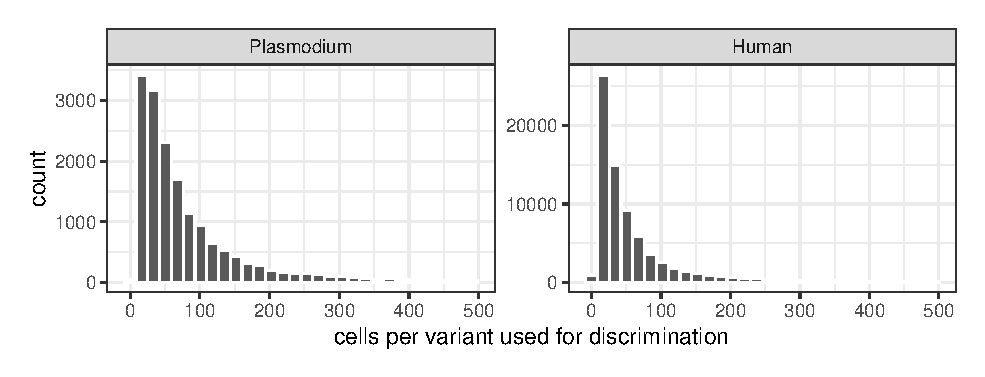
\includegraphics[width=\textwidth]{Cells_per_variant.eps} \label{fig:a}
}\\
%\end{subfigure}
%\begin{subfigure}[b]{\textwidth}
\sidesubfloat[]{
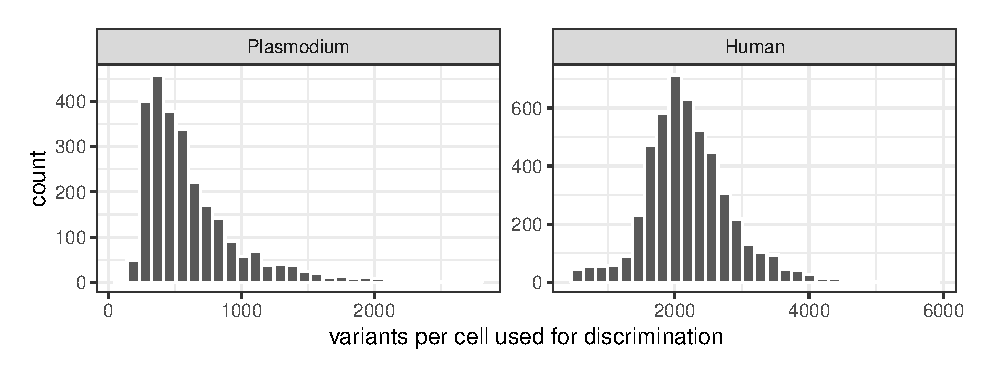
\includegraphics[width=\textwidth]{Variants_per_cell.eps}\label{fig:b}
}
%\end{subfigure}
\par{\textbf{a)} Shows the distribution of number of cells that have each variant and \textbf{b)} shows the distribution of the number of variants expressed by each cell. Both of these are subset to only consider variants that are used for discrimination. A variant is used for discrimination if it has at least four cells expressing the reference allele and four cells expressing the alternative allele.}
\end{centering}
\end{figure}

\par{
To describe the souporcell clustering algorithm, we will start by making some definitions.
}
\\
Definitions
\begin{itemize}
\item $K$: number of genotype clusters to be fixed at the outset. Lower case k will be used for indexing and referring to a specific cluster.
\item $C$: number of cells. Lower case c will be used for indexing and referring to a specific cell barcode. This barcode could have 0, 1, or more cells. It is important for some assumptions in this model that the majority of barcodes contain a single cell. 
\item $L$: number of variant loci. Lower case $l$ will be used to index and refer to a specific locus. We will assume only biallelic variants. $L_c$ will be a list of loci with observed data in cell $c$.
\item $A$: Allele counts. $A_{l,c}$ is a vector of size 2 with the first number representing the number of reference alleles and the second representing the number of alt alleles seen at locus $l$ in cell $c$.
\item $\phi_{k,l}$: cluster center value representing allele fractions of cluster $k$ at locus $l$. This is a real number representing the fraction of ref alleles in this cluster at this locus. We expect this to be near 1.0 (homozygous reference), 0.5 (heterozygous), or 0.0 (homozygous alt) but will be skewed from these values by noise, doublets, and ambient RNA. 
\item $T$: temperature parameter for deterministic annealing process which is described later.

\end{itemize}

\noindent
\subsubsection{Model}

We use a maximum likelihood strategy by maximizing $\mathcal{L}(data)$ under a given model. 
\begin{equation}
\argmax_{\phi} \mathcal{L}(data, \phi)
\end{equation}

We define the likelihood of the data treating cells independently and marginalize each cell across the clusters it could belong to. At each locus the alternate allele count is modeled by a binomial with $n$ as the reference + alternative allele counts for that cell at that locus and $\phi_{k,l}$ as the cluster center value representing the allele fraction for cluster $k$ at locus $l$.

Cluster model Likelihood function

\begin{equation}\label{equation:likelihood}
\mathcal{L}(A) = \prod_{c \in C} \sum_{k \in K} \frac{1}{K} \prod_{l \in L_c} {A_{l,c,0} + A_{l,c,1}  \choose A_{l,c,1}} \phi^{A_{l,c,1}}_{k,l} (1-\phi_{k,l})^{A_{l,c,0}}
\end{equation}
This model deals with sparsity naturally because if a cell has zero reference alleles and zero alternate alleles, a binomial with any probability, zero observations, and zero trials has a probability of one. Instead of uselessly multiplying many ones together, we can ignore sites for which a cell has no alleles.
We could then maximize this likelihood with random initialization of cluster centers $\phi \in (0,1)$ followed by expectation maximization (EM), but there are some problems we can run into.

\subsection{Deterministic Annealing} 
\par{
This method, as is the case with many clustering algorithms, may suffer from local optima in instances of poor initialization of the cluster centers $\phi$. This problem increases dramatically as the number of clusters increase. A standard solution to this problem is to have multiple restarts with random cluster center initializations, but as the number of clusters grows, the number of random restarts necessary to obtain the optimal clustering with high probability is unsustainable\cite{kmeansiterations}\cite{kmeansslow}. In addition to this, the sparse nature of the data increases the potential for local optima in the EM process. The two local optima clustering may produce is when one individual is split across multiple clusters and when multiple individuals are assigned to the same cluster. Some cells will express certain loci and other cells will express other loci. This means that given a random initialization of cluster centers, some cells from individual 1 may initially be more similar to one cluster center and other cells from the same individual may be more similar to a different cluster center because they happened to express different loci and the random initialization happened to fall a particular way. This may lead two cluster centers to be optimized for one individual. Another approach to overcoming local optima in clustering is to initialize the cluster centers intelligently. The most simple initialization strategy is to initialize cluster centers to the values of individual data points (a particular cell in this case) as opposed to randomly in the space, but due to the sparse nature of the data, this would only assign a small minority of the dimensions, the rest of which would need to be random. Other smart cluster center initializations such as kmeans++ are also not particularly applicable to sparse datasets\cite{kmeanspp}. Not having access to these cluster center initialization strategies is limiting and makes it more likely that at initialization, multiple individuals' cells will match a single cluster. Without intelligent cluster center initialization as an option, we turned to methods which are better able to find their way out of local optima. Expectation maximization is known to be less susceptible to local optima as compared to kmeans clustering due to the logsumexp formula which is a smooth maximum (often called softmax) that falls out of marginalizing each data point across all clusters in log space\cite{KHM}. Another clustering algorithm --- K harmonic means --- uses a similar technique choosing the harmonic mean of the distances from a datapoint to all clusters rather than K means' distance to the closest cluster center (the min function) as a loss function to be optimized. The harmonic mean can be thought of as a smooth minimum function. Both of these strategies allow a datapoint to partially affect cluster centers that are not their current best cluster center. Over time, this can lead a cluster center that is not currently the best cluster for many data points to drift towards the ones that are closest to it. As it does so, it may reduce the impact those data points have on another cluster. The combination of these effects tends to improve both of the primary error modes of clustering --- splitting a true cluster across two cluster centers and assigning data points from multiple true clusters to a single cluster center. These soft maximum and soft minimum functions can be thought of as a continuous spectrum of how soft, or smooth, they are -- from min or max to uniform. The shape of these functions between these extremes also matter, but the degree of smoothness tends to matter more. A comparison of these functions can be seen in \ref{figure:softmax}. 
}


\begin{figure}[th!]
\caption{A comparison of smooth minimum and maximum functions}
\label{figure:softmax}
\begin{centering}
%\begin{subfigure}[b]{\textwidth}

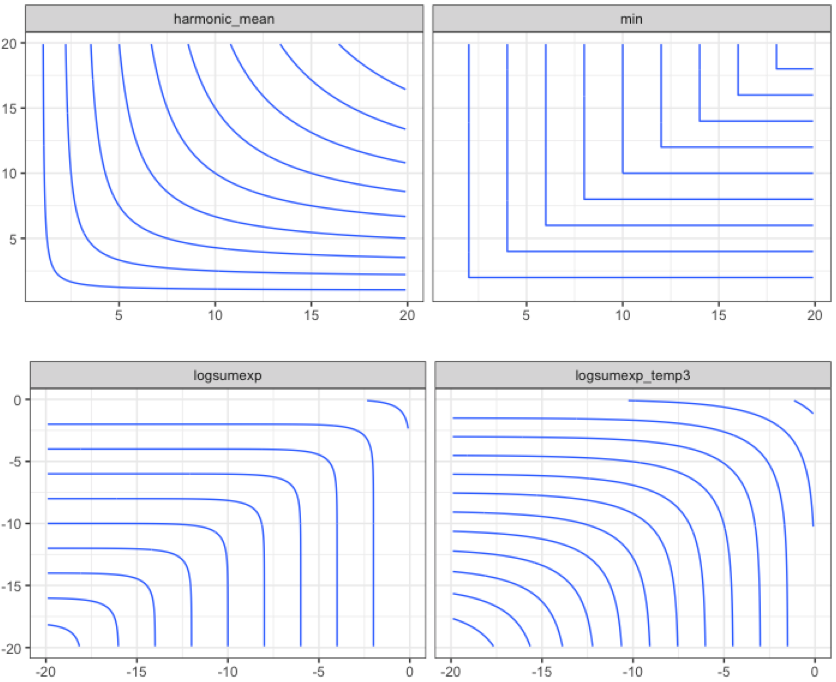
\includegraphics[width=0.75\textwidth]{softmax.png} 
\par{Harmonic mean is smoother than logsumexp, but applying an annealing temperature to logsumexp can make it arbitrarily smooth.}
%\end{subfigure}
%\begin{subfigure}[b]{\textwidth}

%\end{subfigure}
\end{centering}
\end{figure}


\par{
There is another method, deterministic annealing, which allows the degree of how smooth the function is across the optimization process \cite{annealing}\cite{annealing2} (see figure \ref{figure:softmax}). Deterministic annealing, similar to the older and more widely known simulated annealing\cite{simannealing}, takes its namesake from a process in metallurgy in which a metal object is heated to a high temperature and then cooled slowly in a controlled fashion that improves the molecular crystal structures and alters certain properties of the resulting product. They take their mathematical inspiration from statistical mechanics by treating the negative log likelihood as the energy of the system and in an attempt to find the minimum free energy, apply a temperature which begins high and is slowly reduced over time. The temperature dictates the degree of trade-off between exploration of a search space and exploitation of local gradients in the likelihood landscape. Because the problem lends itself to a simple statistical model and deterministic annealing allows us to vary this tradeoff throughout the optimization process, we chose the deterministic annealing variant of expectation maximization for our clustering algorithm. The annealing process requires us to choose a meta-heuristic which is the temperature schedule. In deterministic annealing, the starting temperature is more important than in simulated annealing. With simulated annealing, a high temperature simply means a uniform search over the space regardless of the likelihood landscape. In deterministic annealing applied to clustering, if the temperature starts too high, it makes the data point's posteriors for each cluster uniform. After a few iterations of expectation maximization, the cluster centers may all be nearly identical making the gradients going forward vanishingly small leading to a symmetry breaking local optima. How smooth the soft max function needs to be is a function of the magnitude of the log-likelihoods of each data point, which, in this application, is largely dictated by how many alleles each cell expresses. Through empirical experimentation, we choose to initialize our temperature to one tenth the average number of alleles expressed by each cell. At each temperature step we solve until the change in total log likelihood between steps is minimal (<0.1) which we use as the criteria of convergence. At each new temperature step, the temperature is halved until it is less than one at which point we run a final step at a temperature of one which reduces to the original likelihood function in equation \ref{equation:likelihood}.  We randomly initialize cluster centers and run this optimization 50 times by default and take the solution with the maximum total likelihood. At each temperature step, we define a temperature modified posterior for each cell belonging to each cluster as follows.
}

\begin{equation}
p_T(c \in k) =  \frac{e^{\frac{\log(\mathcal{L}(A_{c,k}))}{T}}}{\sum_{i \in K} e^{\frac{\log(\mathcal{L}(A_{c,i}))}{T}}}
\end{equation}
Which gives our maximization step according to the following equation.
\begin{equation}
\phi_{k,l}' = \frac{\sum_{c \in C} A_{l,c,1} p_T(c \in k)}{\sum_{c \in C}(A_{l,c,1} + A_{l,c,0})p_T(c \in k)}
\end{equation}

\par{
In figure \ref{figure:annealing} you can see that deterministic annealing is better able to find the global optimum likelihood than expectation maximization and that even when it seems to be stuck in a local optimum, as is seen in the log likelihood plateaus in the graph, it is much more likely to find its way out. This becomes much more extreme as the number of individuals, or clusters, there are. And interestingly it also becomes more extreme as the amount of data per cell increases. This may be counter intuitive as you would think the amount of data per cell would make it easier to find the optimal clustering. But instead, the additional data makes the posterior probability for each cell to a cluster be closer and closer to zero or one even at a given random initialization of cluster centers. As the amount of data increases, the log likelihoods are of higher magnitude and the smoothness of the logsumexp function at higher magnitudes is less. The result of this is that it is very common for a given cluster center to be highly preferred over other clusters potentially for multiple individuals' cells and their effect on other clusters to be vanishingly small. This is why it is important both to use deterministic annealing as well as to use the amount of data per cell as a guide for the starting temperature.
}


\begin{figure}[th!]
\caption{EM vs Deterministic Annealing on four and eight individuals}
\label{figure:annealing}
\begin{centering}
%\begin{subfigure}[b]{\textwidth}

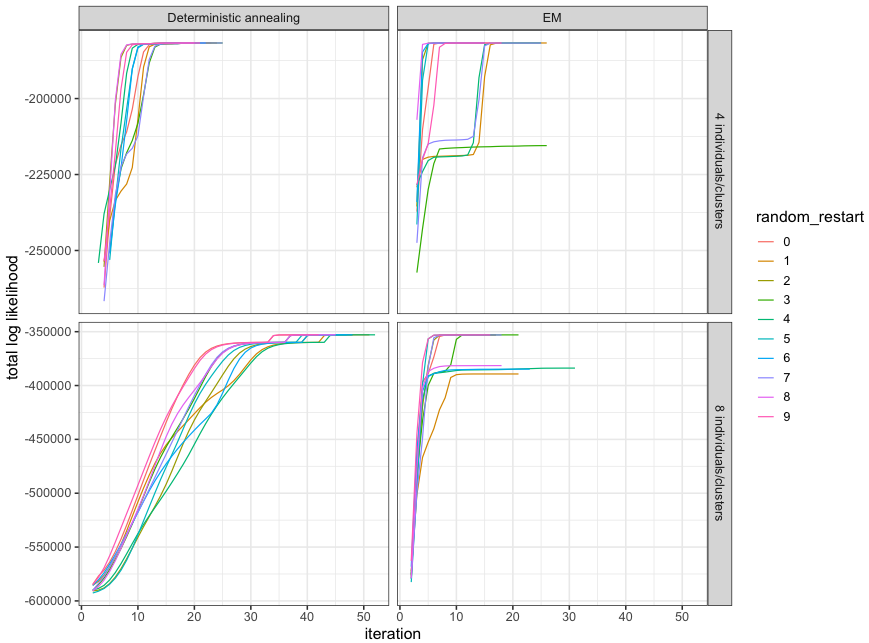
\includegraphics[width=0.75\textwidth]{annealing.png} 
\par{Deterministic annealing finds the optimal clustering (and thus highest likelihood) in all cases whereas EM fails in one random restart with four individuals. With eight individuals, EM fails in several random restarts while Deterministic annealing still finds the optimal clustering every time. This difference becomes much more dramatic with more individuals / clusters.}
%\end{subfigure}
%\begin{subfigure}[b]{\textwidth}

%\end{subfigure}
\end{centering}
\end{figure}


\subsection{Combinatorial experimental design for individual to cluster matching}
\par{
There has been some concern in the community that it will be difficult to know which cluster corresponds to which individual after deconvolution with multiplexed scRNAseq experiments when genotypes are not known a priori. To address this, we propose an experimental design involving m overlapping mixtures for $2m-1$ multiplexed individuals outlined in table \ref{table:multiplex}. Each individual is assigned a binary number $1..2m$, where each bit corresponds to the inclusion (1) or exclusion (0) from each of the mixtures. This gives each individual a unique signature of inclusion/exclusion across the mixtures. Although each sample is in a different number of mixtures, the number of cells per experiment can be adjusted according to the number of mixtures that contain that sample. Souporcell provides a tool to match clusters from two experiments with shared samples.
}



\begin{table}


\caption{Experimental design for matching individuals to clusters}\label{table:multiplex}
\sidesubfloat[]{
\begin{tabular}[htb]{| l | c | c | c |}
%a & & & \\
\hline
Mixture & 1 & 2 & 3 \\
\hline
\hline
Individual a & 0 & 0 & 1 \\ 
\hline
Individual b & 0 & 1 & 0 \\  
\hline
Individual c & 0 & 1 & 1 \\  
\hline 
Individual d & 1 & 0 & 0 \\  
\hline 
Individual e & 1 & 0 & 1 \\  
\hline 
Individual f & 1 & 1 & 0 \\  
\hline 
Individual g & 1 & 1 & 1 \\  
\hline 
\end{tabular}\label{tab:a}}
\hfil
\sidesubfloat[]{
\begin{tabular}[htb]{| l | c | c | c | c |}
\hline
Mixture 1 & d & e & f & g \\
\hline
Mixture 2 & b & c & f & g \\
\hline 
Mixture 3 & a & c & e & g \\
\hline
\end{tabular}\label{tab:b}}
\par{This table outlines an experimental design of seven individuals with three overlapping mixtures to allow for clusters to be assigned to individuals. \textbf{a)} Shows the mapping of individuals to binary numbers where each digit of the binary number represents inclusion/exclusion from a mixture. \textbf{b)} shows the resulting mixtures.}

\end{table}




\subsection{Doublet cell barcode detection}
\par{
One of the major aims of this work is to detect the barcodes which contain multiple cells with different genotypes. 
We do not, however, attempt to detect barcodes which contain multiple cells with the same genotype. We assume that 
the generation of doublet cell barcodes is a random poisson process and that the rate of this poisson process is low enough that 
the chance of droplets with more than two cells are exceedingly unlikely. We view this problem 
as an urn problem in which we each cluster is an urn containing alleles expressed by all of the cells assigned to that cluster. Then we inspect each cell and determine if its alleles were more likely to be drawn from the single best cluster or the allele counts of
the combination of the top two clusters for this cell.
}





Definitions
\begin{itemize}
\item[$A_{k,l}$] Allele counts at locus l for all cells in cluster k according to the maximum probability cluster assignment from our clustering. This is a vector of size two with the ref and alt allele counts.
\end{itemize}

We treat the allele counts of each cell at each locus as random variables drawn from a beta-binomial distribution from either a single cluster or a pair of clusters. The beta-binomial is used to model our uncertainty in the binomial parameter p. For a single cluster the parameters are alpha = 1+alt counts and beta = 1+ref counts. 
For the singleton case, we have 
\begin{equation}
p(c \in K_i) = \prod_{l \in L_c} {A_{l,c,0} + A_{l,c,1}  \choose A_{l,c,1}} \frac{\beta(A_{l,c,0} + 1 + A_{i,l,0}, A_{l,c,1} + 1 + A_{i,l,1})}{\beta(1+A_{i,l,0} + A_{i,l,1})}
\end{equation}


Where $\beta$ is the beta function and cluster $i$ is the best fitting cluster for cell $c$. \\
The expected allele fractions of a doublet coming from cluster $i$, and cluster $j$ is the average of the allele fractions of the two clusters. To obtain the pseudocounts needed to parameterize the beta-binomial, we use the total counts of the cluster with less coverage at this locus. That is, 
\begin{equation}
alpha_{l,i,j} = 1 + \frac{\frac{A_{i,l,0}}{A_{i,l,0}+A_{i,l,1}} + \frac{A_{j,l,0}}{A_{j,l,0}+A_{j,l,1}}}{2}min(A_{i,l,0}+A_{i,l,1}, A_{j,l,0}+A_{j,l,1})
\end{equation}

\begin{equation}
beta_{l,i,j} = 1 + \frac{\frac{A_{i,l,1}}{A_{i,l,0}+A_{i,l,1}} + \frac{A_{j,l,1}}{A_{j,l,0}+A_{j,l,1}}}{2}min(A_{i,l,0}+A_{i,l,1}, A_{j,l,0}+A_{j,l,1})
\end{equation}
The doublet probability given those conservative parameters becomes
\begin{equation}
p(c \in K_i \cup K_j) = \prod_{l \in L_c}  {A_{l,c,0} + A_{l,c,1}  \choose A_{l,c,1}}\frac{\beta(A_{l,c,0} + alpha_{l,i,j}, A_{l,c,1} + beta_{l,i,j})}{\beta(alpha_{l,i,j} + beta_{l,i,j})}
\end{equation}
The posterior for each cell being a doublet is then given by
\begin{equation}
p(doublet_c | c) = \frac{p(c \in K_i \cup K_j)p(doublet)}{p(c \in K_i \cup K_j)p(doublet) + p(c \in K_i)(1-p(doublet))}
\end{equation}
Where cluster i is the best fitting cluster for cell $c$ and cluster $j$ is the second best fitting cluster for cell $c$. We allow the prior to be set by the user but have used an uninformed prior of 0.5 for all of our analysis. \\
We run the above process and remove doublet cells from the cluster allele counts repeatedly until we no longer find new doublets. \\ \\





\subsection{Ambient RNA detection and Cluster genotype coinference}
One major goal of clustering scRNAseq by genotypes is calling the genotypes for each individual / cluster.
But as previously discussed, there can be lysed cells in solution prior to cell partitioning which contribute a background noise to both genotypes and transcriptional profiles. 
This ambient RNA gives a fuzzy picture of the transcriptional profile and makes cluster genotypes which are in truth homozygous appear heterozygous. 
Luckily with genotype mixtures, we can use our prior knowledge of the ploidy of the mixed organisms along with our genotype cluster assignments to 
make a co-inference of both the genotypes and level of ambient RNA in the experiment.

\subsubsection{Mixture model of ambient RNA and cell RNA}
Definitions
\begin{itemize}
\item $\rho$: probability any given allele is arising from ambient RNA as opposed to from the cell associated with that barcode. This will be learned.
\item $P$: ploidy. We assume ploidy is limited to 1 or 2.
\item $A_l$: total allele expression at locus l. This is again a vector of length 2 denoting the reference and alternative allele counts.
\item $g$: used to denote the number of copies of the reference allele. The expected reference allele rate without ambient RNA is g and g is an integer value [0..P]. Note that for biallelic variants and ploidy 1 or 2, g is sufficient to uniquely determine the genotype. 
\item $p(true)$: prior for variant being a true variant vs a false positive. The default is 0.9 which was the value used for all analyses.
\end{itemize}


Once again we solve this with a maximum likelihood approach.
\begin{equation}
\argmax_{\rho} p(data, \phi)
\end{equation}

Here, the proportion of ambient RNA in the system, $\rho$, is the only free parameter and we solve for it using maximum likelihood. The model treats each locus in each cluster as coming from one of three genotypes for diploid (0/0, 0/1, 1/1, here denoted by g = 0, 1, or 2) and two genotypes from haploid (0, 1). We treat each cluster as independent and each locus as independent, before marginalizing across the possible genotypes. The model also considers the possibility of the variant being a false positive. In this case, the variant will not segregate into distinct allele frequencies between different clusters and it will most likely not attain a value close to the standard allele frequencies expected from the diploid or haploid genotypes. Thus, we model the allele counts in each cluster as having come from a mixture of ambient RNA (an average allele fraction in the experiment) and from the cells in that cluster. The observed allele fractions are assumed to have been drawn from a binomial distribution with a probability that was skewed away from $p = g/P$ by the level of ambient RNA $\rho$. Thus, the probability of the binomial from which the allele counts are drawn for true positive variants is the following.



\begin{equation}
p_{tp} = (1-\rho)\frac{g}{P} + \rho \frac{A_{l,0}}{A_{l,0}+A_{l,1}}
\end{equation}
For a false positive the parameter is
\begin{equation}
p_{fp} = \frac{A_{l,0}}{A_{l,0} + A_{l,1}}
\end{equation}

Thus, the full model is
\begin{equation}
%\begin{multline}
\begin{split}
p(data | \rho)  &= \prod_{l \in L} \bigg[p(true) \prod_{k \in K} \sum^P_{g=0} \frac{1}{P}  {A_{l,c,0} + A_{l,c,1}  \choose A_{l,c,1}} p_{tp}^{A_{k,l,0}} (1-p_{tp})^A_{k,l,1}  \\ &+ (1-p(true)) \prod_{k \in K} {A_{l,c,0} + A_{l,c,1}  \choose A_{l,c,1}} p_{fp}^{A_{k,l,0}} (1-p_{fp})^A_{k,l,1} \bigg]
%\end{multline}
\end{split}
\end{equation}



And the model treats each locus in each cluster as coming from one of three genotypes for diploid (0/0, 0/1, 1/1, here denoted by g=0,1, or 2) and two genotypes from haploid (0, 1). We 
treat each cluster as independent and each locus as independent. Then we marginalize across the possible genotypes.  
And so we model the allele counts in this cluster as having come from 
a mixture of ambient RNA and from this cells in this cluster. And then we model the observed allele fractions as being drawn from a binomial distribution 
with a probability which was skewed away from $p=\frac{g}{P}$ by the level of ambient RNA. And we believe that the ambient RNA is drawn from 
an average of all of the reads in the experiment. As such, the expected allele fraction coming from the soup is $\frac{A_{l,0}}{A_{l,0} + A_{l,1}}$. 
Thus, the probability of the binomial of the mixture of cell data is the following.
\begin{equation}
p_{tp} = (1-\rho)\frac{g}{P} + \rho \frac{A_{l,0}}{A_{l,0}+A_{l,1}}
\end{equation}
\begin{equation}
p_{fp} = \frac{A_{l,0}}{A_{l,0}+A_{l,1}}
\end{equation}



Now we use that binomial probability in the full likelihood.
\begin{equation}
\begin{split}
p(data | \rho) = \prod_{l \in L} \bigg[ & p(true) \prod_{k \in K} \sum_{g = 0}^P \frac{1}{P} \binom{A_{k,l,0} + A_{k,l,1}}{A_{k,l,0}} p_{tp}^{A_{k,l,0}} (1-p_{tp})^{A_{k,l,1}} \\
 & + (1-p(true))\prod_{k \in K}\binom{A_{k,l,0} + A_{k,l,1}}{A_{k,l,0}}p_{fp}^{A_{k,l,0}} (1-p_{fp})^{A_{k,l,1}}  \bigg]
\end{split}
\end{equation}

\subsubsection{Inference}
We solve for $\rho$ with gradient descent using the statistical modeling domain specific language STAN. Next, we calculate the posterior of the variant being a true positive for each of the three (or two in the haploid case) genotypes versus it being a false positive. The prior on variants being true positives can be set by the user, but defaults to 0.9 which is the value used in our analyses.




%********************************** %Second Section  *************************************
\section{Results}



\subsection{Benchmarking: Synthetic human cell mixture}

Currently, there are no good generative models available for batch effects, allele-specific expression, ambient RNA, and doublets in scRNAseq that can be used to generate in silico data for testing methods that cluster by genotype. To generate realistic data with known ground truth we sequenced five lines of induced pluripotent stem cells (iPSCs) from the Human iPSC initiative\cite{hipsci} with the 10x Chromium single cell system, both individually and in a mixture of all five lines (with three replicates of the mixture). Each mixture contained 5-7,000 cells and ~25,000 UMIs per cell. We first synthetically mixed 20\% of the cells from the 5 individual samples while retaining their sample of origin. To make the synthetic mixture as close to real data as possible, we also simulated 6\% doublets by switching all of the reads' barcodes from one cell to that of another cell and 5\% ambient RNA by randomly switching cell barcodes for 5\% of the reads. A low dimensional representation of the expression matrix reveals relatively little variation, as expected, since there is only one cell type present (\ref{figure:synthetic}a). Indeed, the most significant driver of expression appears to be the donor of origin, but the donor cells overlap in expression patterns and it is not possible to assign a donor to each cell based solely on expression patterns.



\begin{figure}[th!]
\caption{Synthetic human mixture}
\label{figure:synthetic}
\begin{centering}

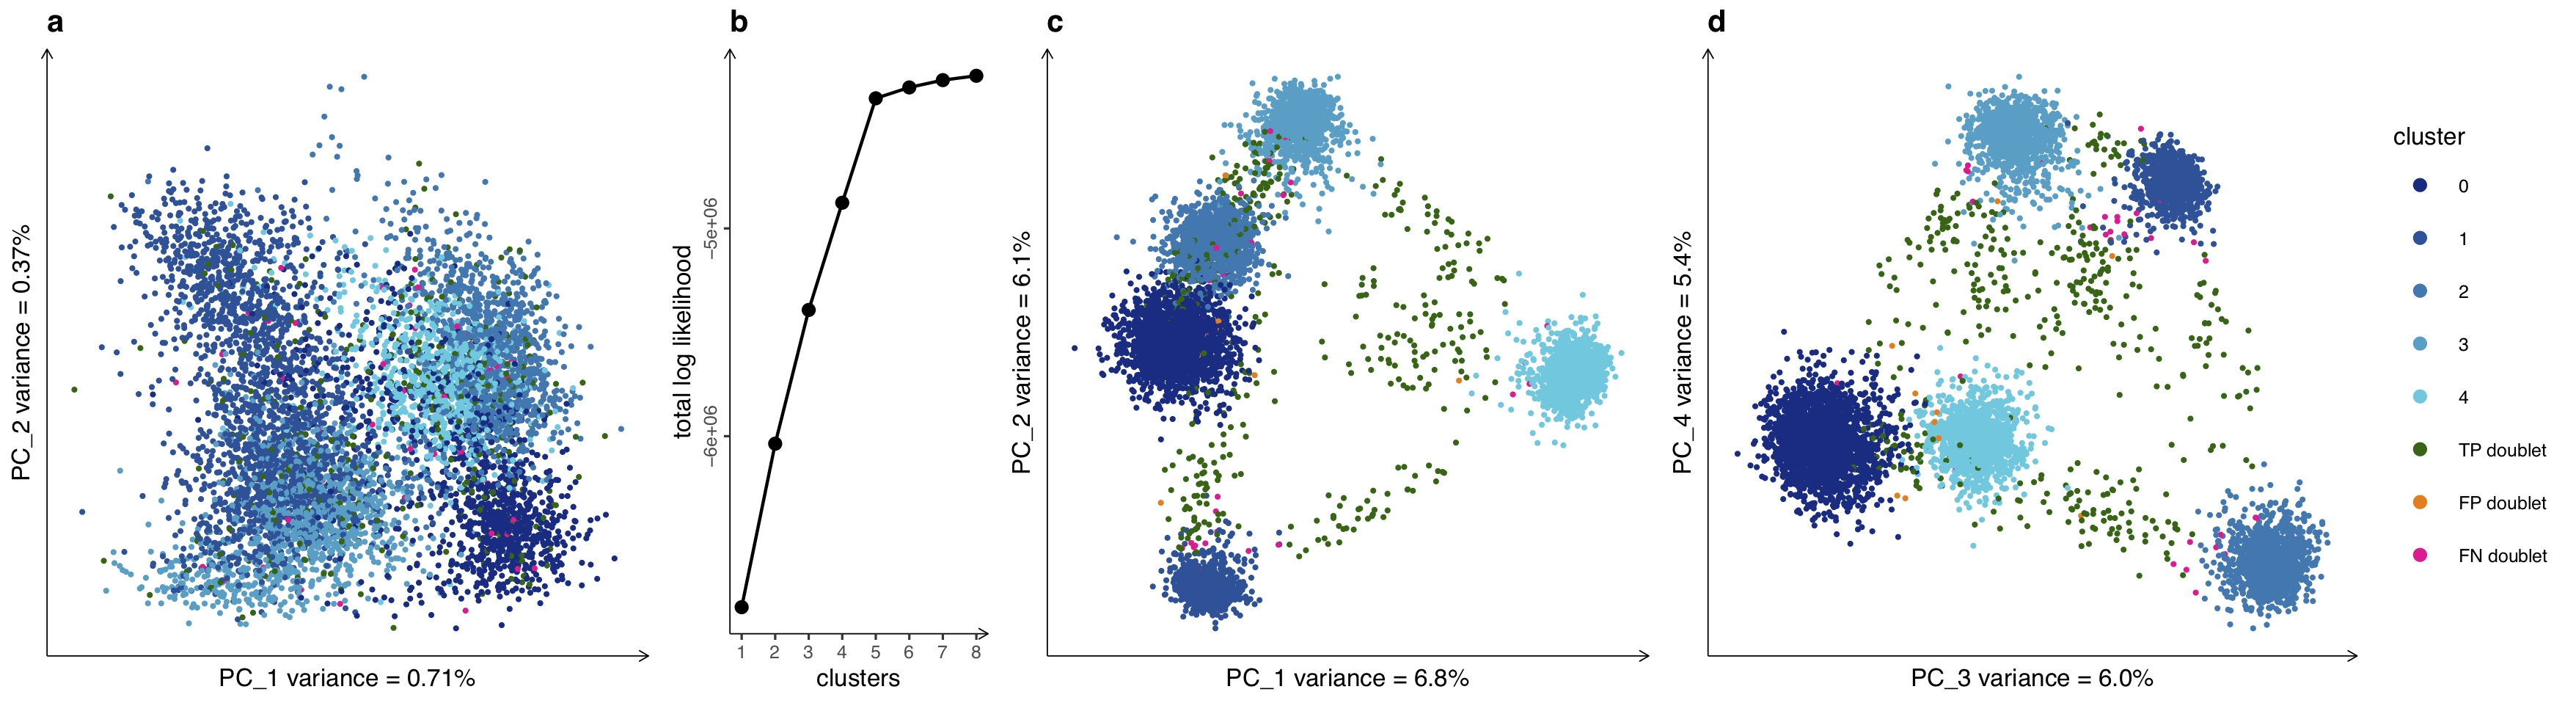
\includegraphics[width=\textwidth]{simulated.jpg} 
\par{\textbf{a)} Expression PCA of a synthetic mixture cells from five HipSci cells lines (n=7073 cells) with 5\% ambient RNA and 6\% doublets colored by known genotypes. Because these samples only contain one cell type, the largest remaining source of variation in the expression profile comes from the genotype, although the signal is not sufficient for accurate genotype clustering. \textbf{b)} Elbow plot of the number of clusters versus the total log likelihood showing a clear preference for the correct number of clusters (k=5). \textbf{c} and \textbf{d)} PCA of the normalized cell-by-cluster log likelihood matrix from souporcell (n=7073 cells). As this is a synthetic mixture in which we know the ground truth, we color by genotype clusters and highlight errors in orange (false positive doublets) and pink (false negative doublets).}

\end{centering}
\end{figure}





\subsection{Benchmarking: Real human cell mixture}

Next we compare to a true mixture of human cells in which we do not have full ground truth. The results (shown in \ref{figure:real} are strikingly similar to those in \ref{figure:synthetic} which suggest that our synthetic mixture is realistic. And to show that this is replicable, we show the same plots on two experimental replicates of this mixture (see figure \ref{figure:humanreplicates}).

\begin{figure}[th!]
\caption{Experimental human mixture}
\label{figure:real}
\begin{centering}

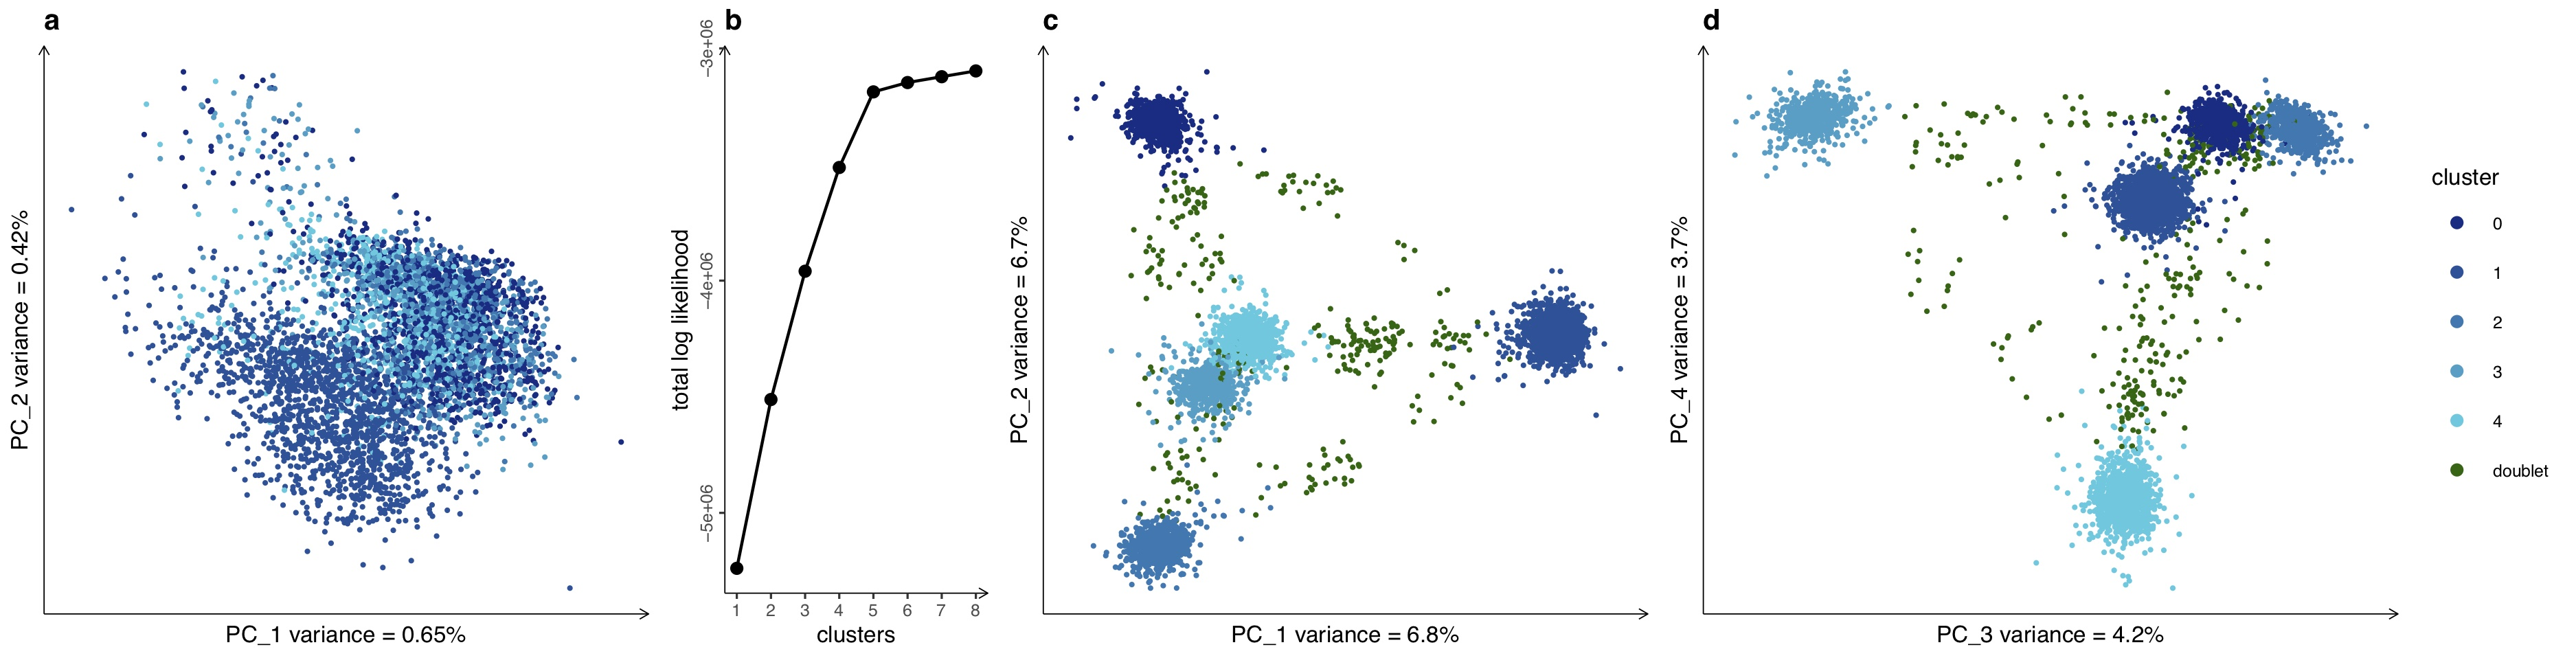
\includegraphics[width=\textwidth]{realmix.jpg} 
\par{\textbf{a)} Expression PCA of a single replicate (see Fig. S1 for reps) of the experimental mixtures (n=4925 cells) colored by genotype clusters from souporcell. \textbf{b)} Elbow plot of the total log likelihood versus different numbers of clusters showing a clear preference for the correct number of clusters. \textbf{c} and \textbf{d)} PCA showing the first four PCs of the normalized cell-by-cluster log likelihood matrix colored by cluster (n=4925 cells).}
\end{centering}
\end{figure}


%\begin{figure}[th!]
%\caption{Experimental human mixture replicates}
%\label{figure:humanreplicates}
%\begin{centering}

%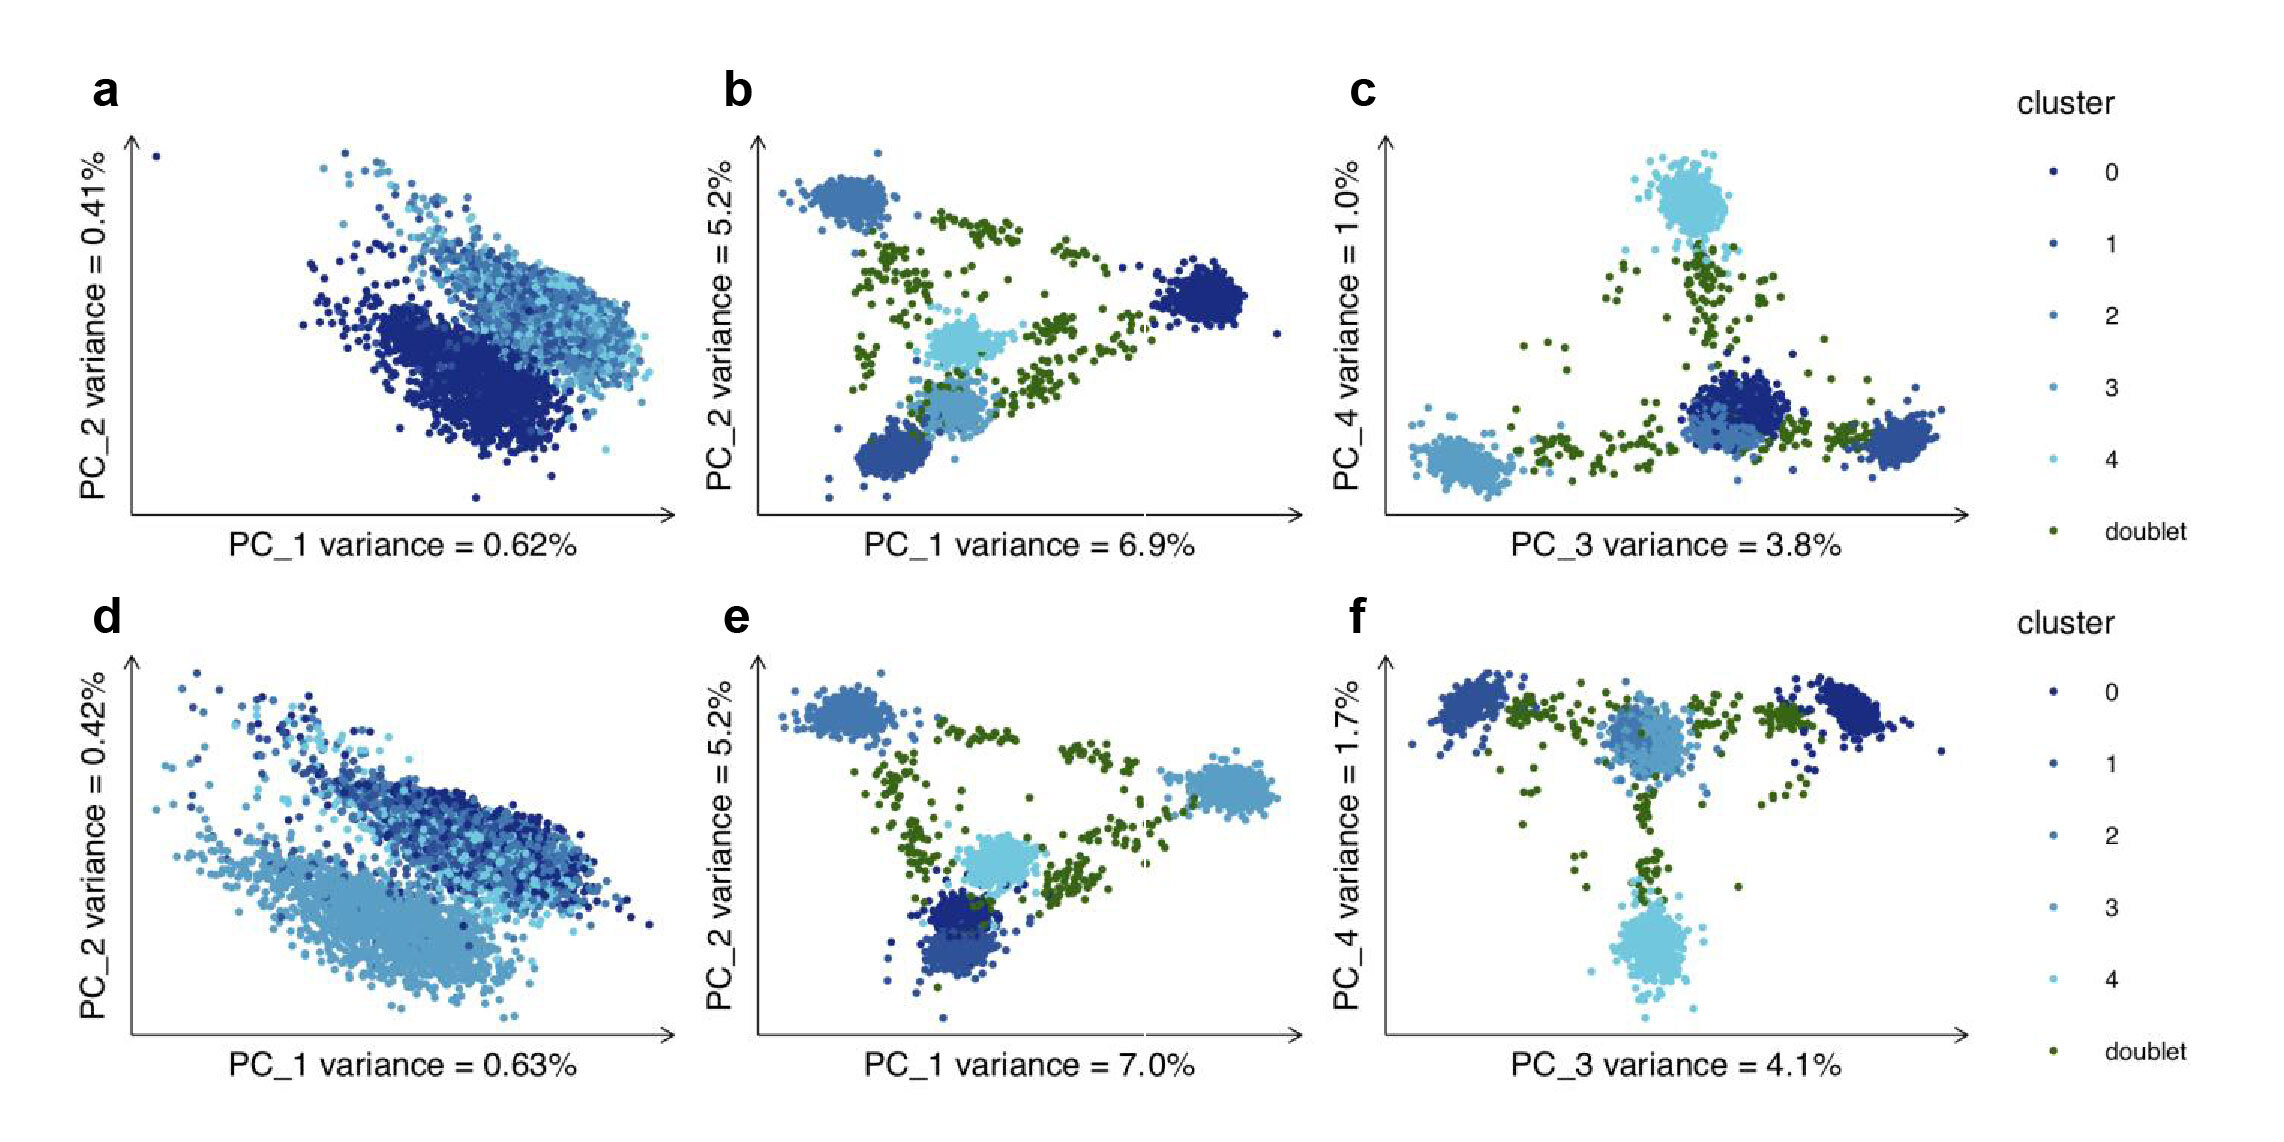
\includegraphics[width=\textwidth]{human_replicates.jpg} 
%\par{\textbf{a)} Expression PCA of a single replicate (see Fig. S1 for reps) of the experimental mixtures (n=4925 cells) colored by genotype clusters from souporcell. \textbf{b)} Elbow plot of the total log likelihood versus different numbers of clusters showing a clear preference for the correct number of clusters. \textbf{c} and \textbf{d)} PCA showing the first four PCs of the normalized cell-by-cluster log likelihood matrix colored by cluster (n=4925 cells).}
%\end{centering}
%\end{figure}


\subsection{Benchmarking: demuxlet paper dataset}

\par{
In order to demonstrate souporcell on an external and widely used benchmark dataset, we downloaded the
three overlapping mixtures from the demuxlet paper\cite{demuxlet}
. Sample A contains a mixture of four donors?
PBMCs, Sample B contains a mixture of four different donors? PBMCs, and Sample C contains a mixture
of all 8 donors? PBMCs. We synthetically combined this data into a single dataset and clustered with
souporcell. Figure \ref{figure:demuxlet}a shows that the resulting clusters either contain cells from Sample A or Sample B,
but not both as is expected from this experimental setup. We also show that the first cluster of the doublet
assignments are also largely consistent with this experimental design (figure \ref{figure:demuxlet}b). 
}

\begin{figure}[htbp!]
\caption{Demuxlet data}
\label{figure:demuxlet}
\begin{centering}
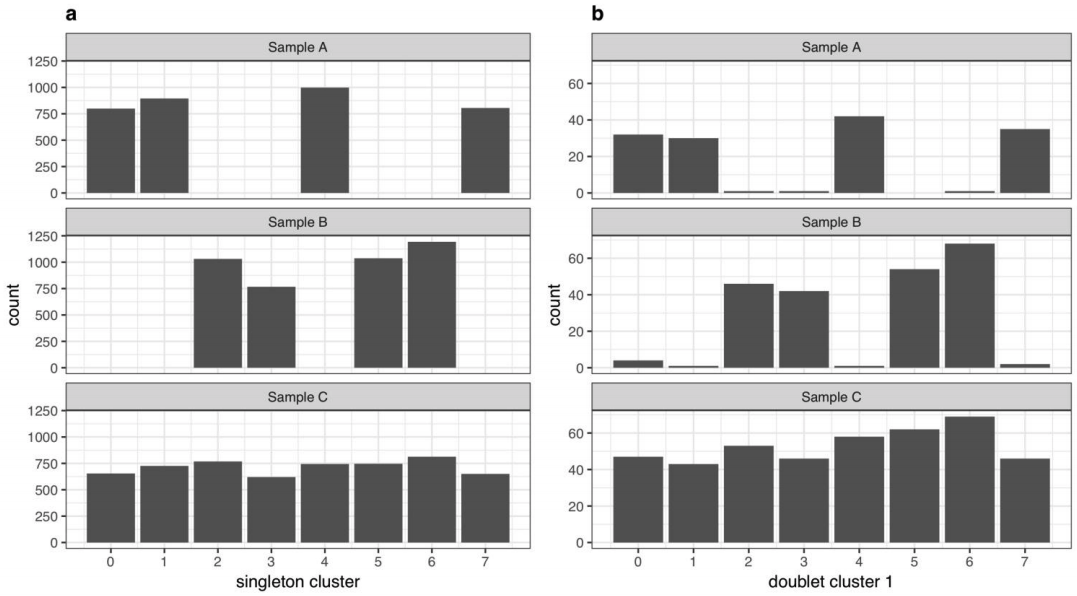
\includegraphics[width=\textwidth]{demuxletdata.png} 
\par{\textbf{a)} souporcell cluster assignments of singletons for combined dataset showing that Sample A and Sample B are non-overlapping and
Sample C contains all 8 samples. \textbf{b)} shows the first cluster of the doublet assignment for doublets showing largely non-overlapping
assignments between Samples A and B.}
\end{centering}
\end{figure}

\subsubsection{Deconvolution of overlapping mixtures}

\par{
To enable identification of which cluster is which individual using the overlapping mixture experimental
design outlined in Table 1, we provide a tool shared\_samples.py which takes as input two souporcell
output directories and the number of samples which are shared. It compares the sum of squared
differences of the allele fraction of confident (>95\% confident genotype call in all clusters) shared variant
calls between clusters in the two experiments and outputs the best matches for the number of shared
samples. We tested this using multiple different runs of souporcell on the synthetic mixture of 5 HipSci
cell lines with 6\% doublets and 5\% ambient RNA and gave both as input to the shared\_samples.py tool
and it correctly assigned the clusters in one run to the clusters in the second experiment which
corresponded to the same samples. We also ran souporcell on the three demuxlet datasets separately and
ran the shared\_samples.py tool on Sample A vs Sample C and Sample B vs Sample C and it confidently
identified the non-overlapping clusters in Sample C which correspond to A and B. 
}



\subsubsection{Validation and comparison to other methods}

We compared souporcell to vireo and scSplit, two other tools that do not require prior genetic information. First, we ran variant calling and cell allele counting as recommended for each tool. Using souporcell, we clustered cells by their genotypes, and evaluated the correct number of clusters through an elbow plot comparing the total log probability versus a varying number of clusters (\ref{figure:synthetic}b). The clustering output can be viewed as a matrix with cells as rows and clusters as columns with the values being the log likelihood of that cell versus the corresponding cluster. To visualize the five clusters identified by genotype we carried out a Principal Component Analysis (PCA) of the normalized log likelihood matrix, which reveals a clear separation of the clusters, with interspersed doublets (\ref{figure:synthetic}c and d).  For these data souporcell assigned 6612/6622 singletons and 415/451 doublets correctly; four singletons were falsely labeled as a doublet, 35 doublets were misidentified as singletons, and one doublet and four singletons were unassigned. We carried out the same analysis for the three replicates of the  experiment mixtures and show results for one (\ref{figure:real}). The expression PCA (Fig. 2e) and normalized cell-cluster loss PCA (\ref{figure:real}c,d) of the experimental mixture were similar to the synthetic mixture indicating that the synthetic mixtures were an accurate approximation of real mixtures. To compare doublet detection between methods, we calculated a receiver-operator characteristic (ROC) curve of the doublet calls (\ref{figure:compare}i) on a synthetic mixture with 6\% doublets and 10\% ambient RNA that showed the area under the curve values of 0.98 and 0.91 for souporcell and vireo, respectively. We also show point estimates for the doublet threshold chosen. Demuxlet's posterior doublet probability output did not have enough significant digits and is 1.0 until it starts varying with 27\% false positives. The default doublet probability threshold for demuxlet gives nearly 40\% false positive doublets.

\par{
Each of the five human iPSC lines has existing WGS data generated as part of the HipSci Project\cite{hipsci2}. Therefore, for the experimentally mixed replicates, we compared each tool's clustering to sample assignments obtained from demuxlet using genotypes available from the WGS. Demuxlet significantly overestimates doublets versus expectations based on the number of cells loaded\cite{10xsinglecell} especially as ambient RNA increases (\ref{figure:compare}b). Because we could not trust the doublet calls of demuxlet, we allowed scSplit, vireo, and souporcell to exclude their called doublets and then compared the remaining cells to demuxlet's best single genotype assignment. The Adjusted Rand Index (ARI) of the remaining cell assignments versus demuxlet were 1.0 (fully concordant) for souporcell and vireo across the three replicates and an average of 0.97 for scSplit.
}

\par{
To evaluate the robustness of each tool across a range of parameters, we created synthetic mixtures of the five individual human iPSC scRNAseq experiments to test both the sensitivity to the ambient RNA level (\ref{figure:compare}b,c) and the ability to accurately assign cells to a cluster if it is much smaller than other clusters (\ref{figure:compare}d). For the ambient RNA experiment, we synthetically combined 20\% of the cells from each of the five individual samples and simulated 6\% intergenotypic doublets and a range of ambient RNA from 2.5\%-50\% representing realistic ranges previously reported\cite{soupx}. We found that souporcell and vireo retain high accuracy with souporcell being more robust at accurately calling doublets in high ambient RNA cases (\ref{figure:compare}c). The ARI of scSplit and demuxlet suffered due to poor doublet detection. With these data we also show that souporcell is able to accurately estimate the amount of ambient RNA in the experiment (\ref{figure:compare}c). To test robustness to sample skew, e.g., one donor's cells are underrepresented, we created a set of synthetic mixtures with 1,000 cells from each of four individual samples and 25-800 cells for the minority cluster including 8\% ambient RNA and 6\% doublets (\ref{figure:compare}d). We found that all tools performed well down to the minority cell cluster comprising only 1.2\% (50 cells) of total cells (Fig. 2m), but only souporcell and vireo were able to correctly identify all minority sample singletons as their own cluster down to 0.6\% of all cells. Again, demuxlet's poor ARI was due primarily to extremely high levels of false positive doublets (\ref{figure:compare}a).
}


\begin{figure}[htbp!]
\caption{Comparison to competing methods}
\label{figure:compare}
\begin{centering}

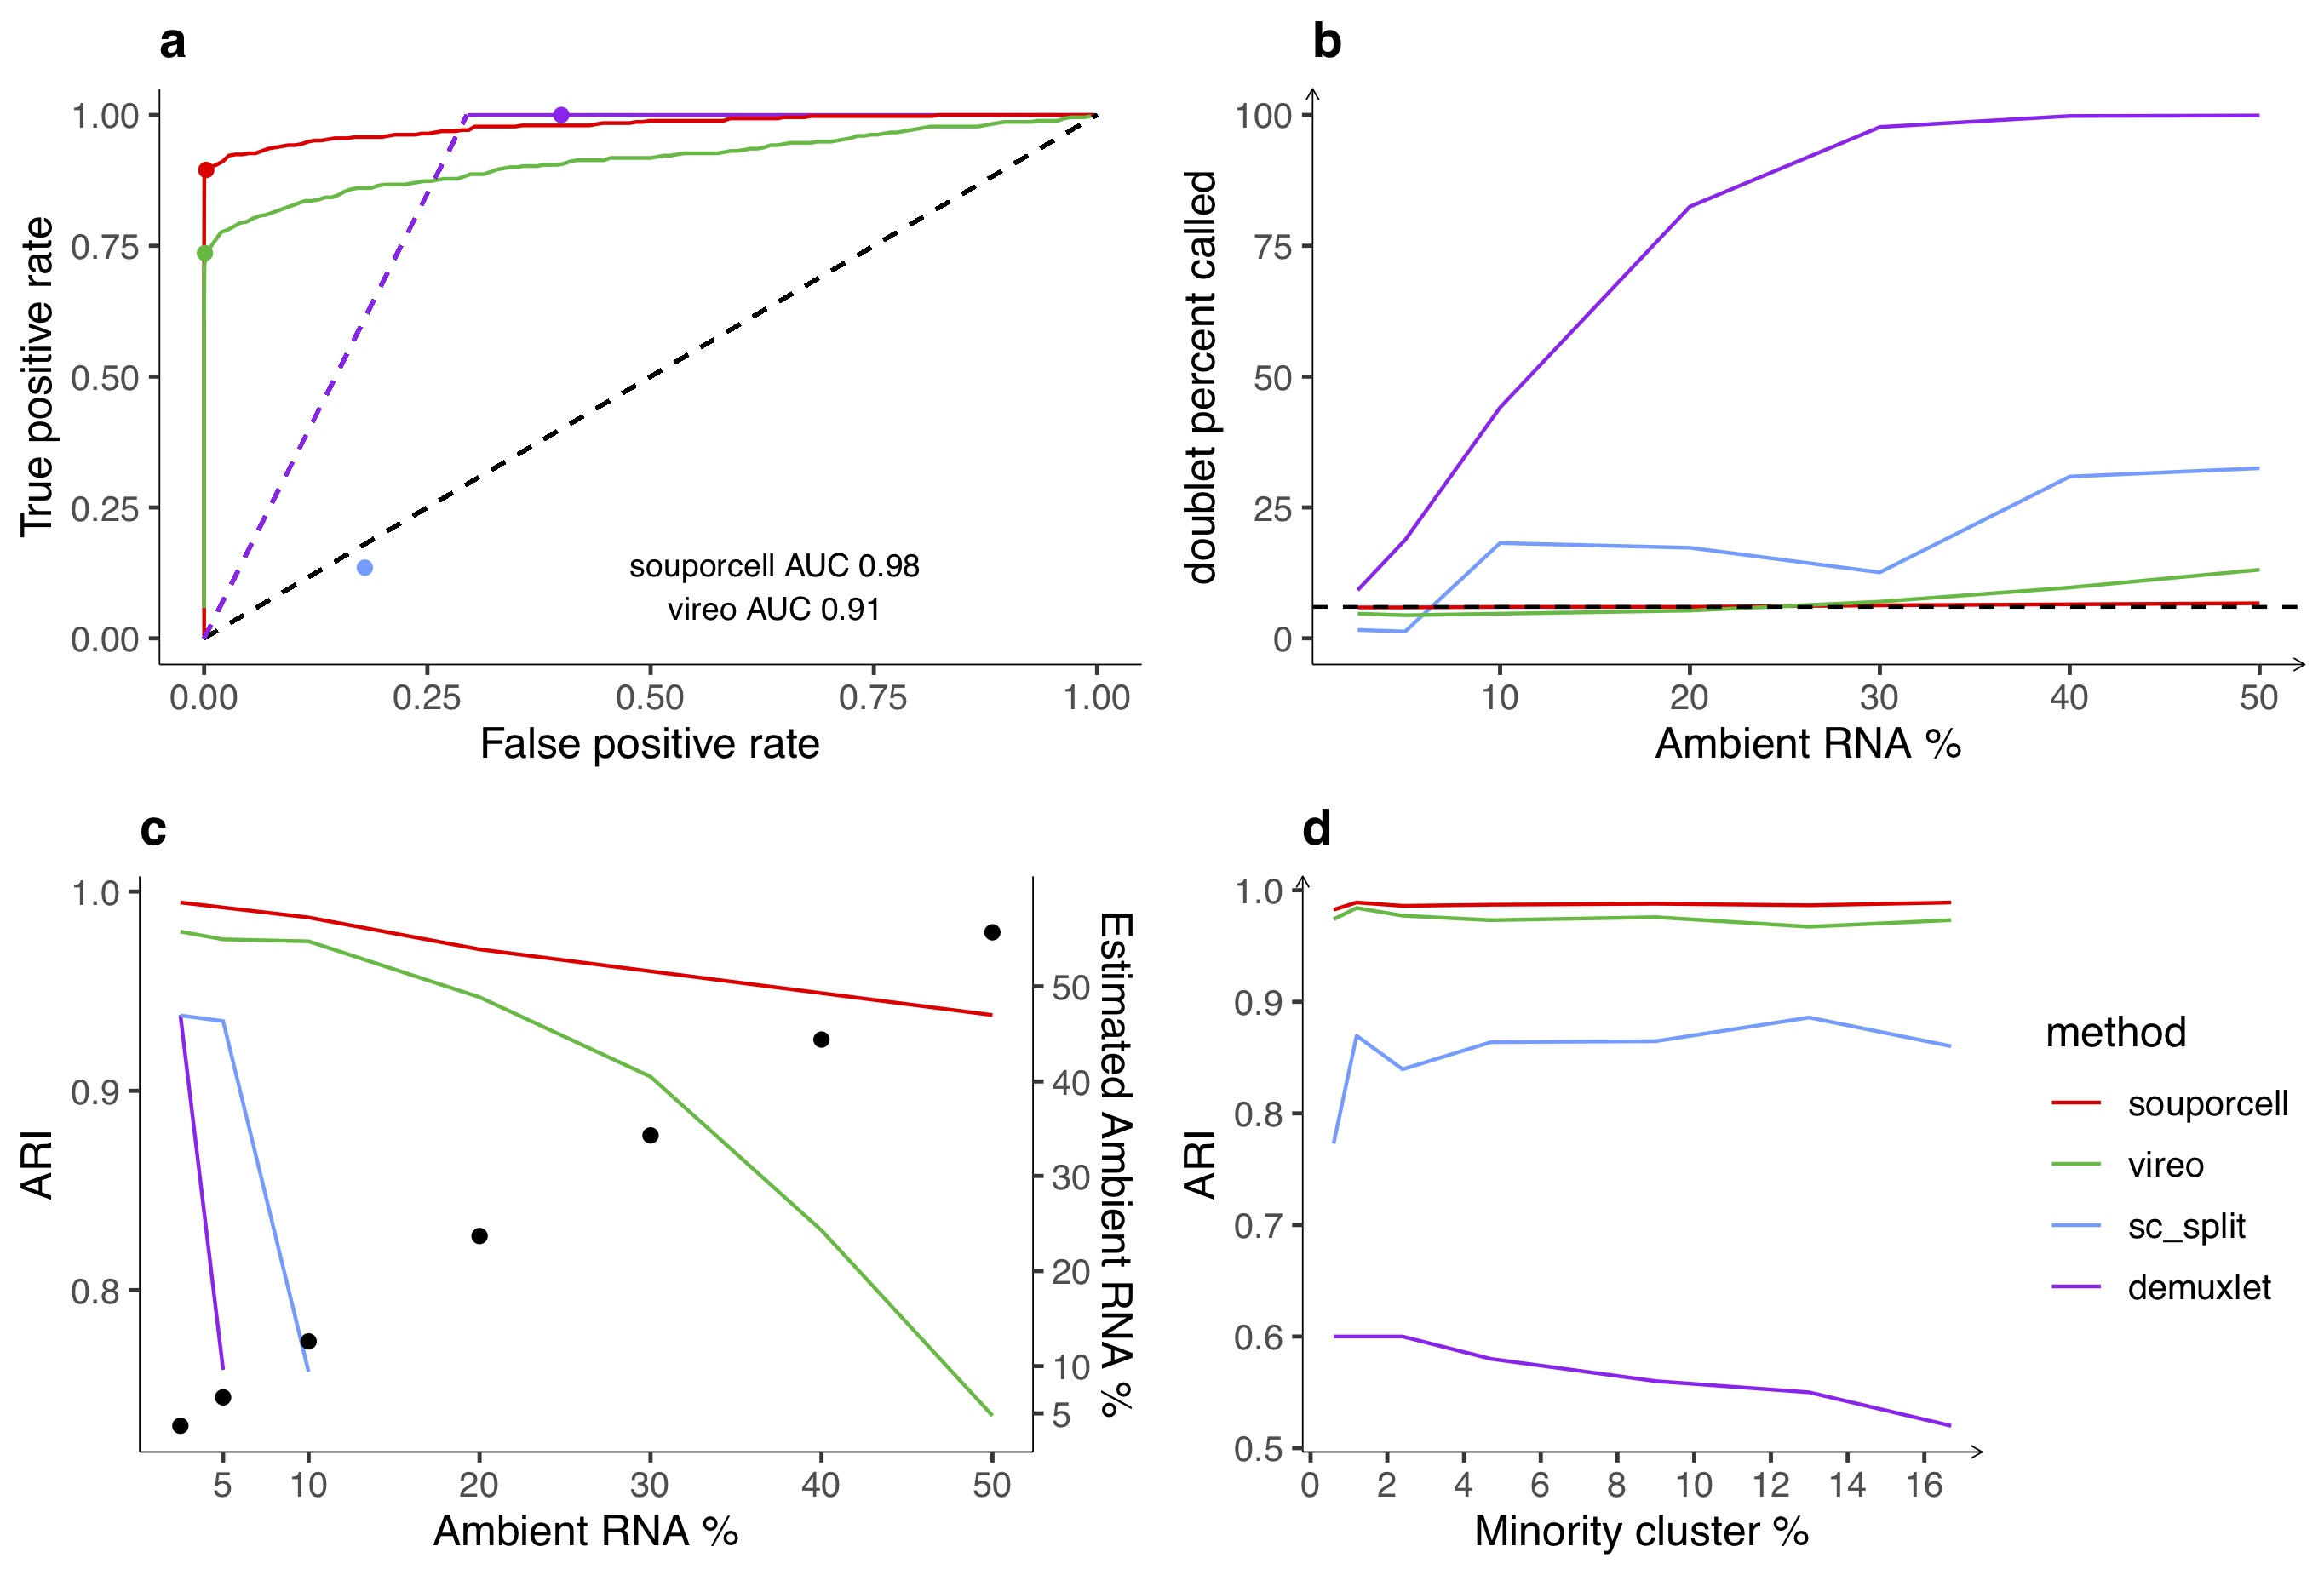
\includegraphics[width=\textwidth]{humcompare.jpg} 
\par{\textbf{a)} ROC curve of the doublet calls made by souporcell and vireo and a point estimate for scSplit (blue dot) for a synthetic mixture with 6\% doublets 451/7073 and 10\% ambient RNA. We show both the curves and the threshold chosen (points) for each tool. scSplit did not give a score so we simply show the point estimate. Demuxlet's doublet probabilities were all 1.0 until the solid line starts, so we show a theoretical dotted line up to that point. \textbf{b)} Doublet call percentages for all tools on synthetic mixtures for varying amounts of ambient RNA versus the actual doublet rate (dotted line). \textbf{c)} Adjusted Rand Index (ARI) versus the known ground truth of synthetic mixtures with 6\% doublets and a varying amount of ambient RNA. For levels >=10\% ambient RNA, scSplit identified one of the singleton clusters as the doublet cluster, which means that the ARI was not clearly interpretable. Right y-axis vs points shows the estimated ambient RNA percent by souporcell versus the simulated ambient RNA percent. \textbf{d)} ARI of each tool on a synthetic mixture with 8\% ambient RNA and 6\% doublet rate with 1,000 cells per cluster for the first four clusters and a variable number of cells in the minority cluster (25-800 cells in the minority cluster).}

\end{centering}
\end{figure}

\par{
We then compared souporcell's genotype and ambient RNA co-inference to vireo and scSplit versus the variants called from whole genome sequencing data. In scRNAseq data most variants have very low coverage per cluster compared to what would be generated from WGS data, thus the genotype accuracy is significantly lower than one would attain with genome sequencing. Nevertheless, souporcell surpasses both vireo and scSplit in genotype accuracy on a synthetically mixed sample with 6\% doublets and 10\% ambient RNA. The most common error mode for vireo and scSplit is calling homozygous reference loci as heterozygous variants  which is expected when ambient RNA is not accounted for, as it is not in these two tools.
}



\subsection{Maternal-Fetal data}

\par{
Next, we considered more challenging scenarios involving multiple cell types, widely varying numbers of cells per sample, and closely related genotypes. The decidua-placental interface plays an important role in pregnancy and birth, and is of importance to several diseases, including pre-eclampsia\cite{maternalfetal}. Recently, more than 70,000 cells were profiled by scRNAseq\cite{nkhla} to explore the transcriptional landscape at this interface. The decidua is primarily composed of maternal cells with some invading fetal trophoblasts, while the placenta is largely composed of cells of fetal origin with the exception of maternal macrophages. In the study exploring this interface\cite{maternalfetal}, WGS from blood and placenta was used to genotype both mother and fetus, and demuxlet was used to assign cells to each individual. Here, we applied souporcell, vireo, and scSplit to two placental samples and one decidual sample from a single mother to determine if cellular origins could be established without reference genotypes. We show the expression t-SNE of a single placental sample labeled by cell type annotation\cite{maternalfetal} and colored by genotype cluster as assigned by each method (\ref{figure:maternal}). While souporcell clusters agree with demuxlet and segregate with the expected cell type clusters, vireo and scSplit have major discordances with demuxlet. This is similar for the other samples tested. Comparing souporcell to demuxlet, there are 21 cells that demuxlet labels as maternal or fetal but which appear in the other individual's cell type clusters. Based on the position of these cells in the expression t-SNE plot, it is most likely that these are errors in the demuxlet assignments that are not made by souporcell. 
}


\begin{figure}[htbp!]
\caption{Maternal/fetal data}
\label{figure:maternal}
\begin{centering}

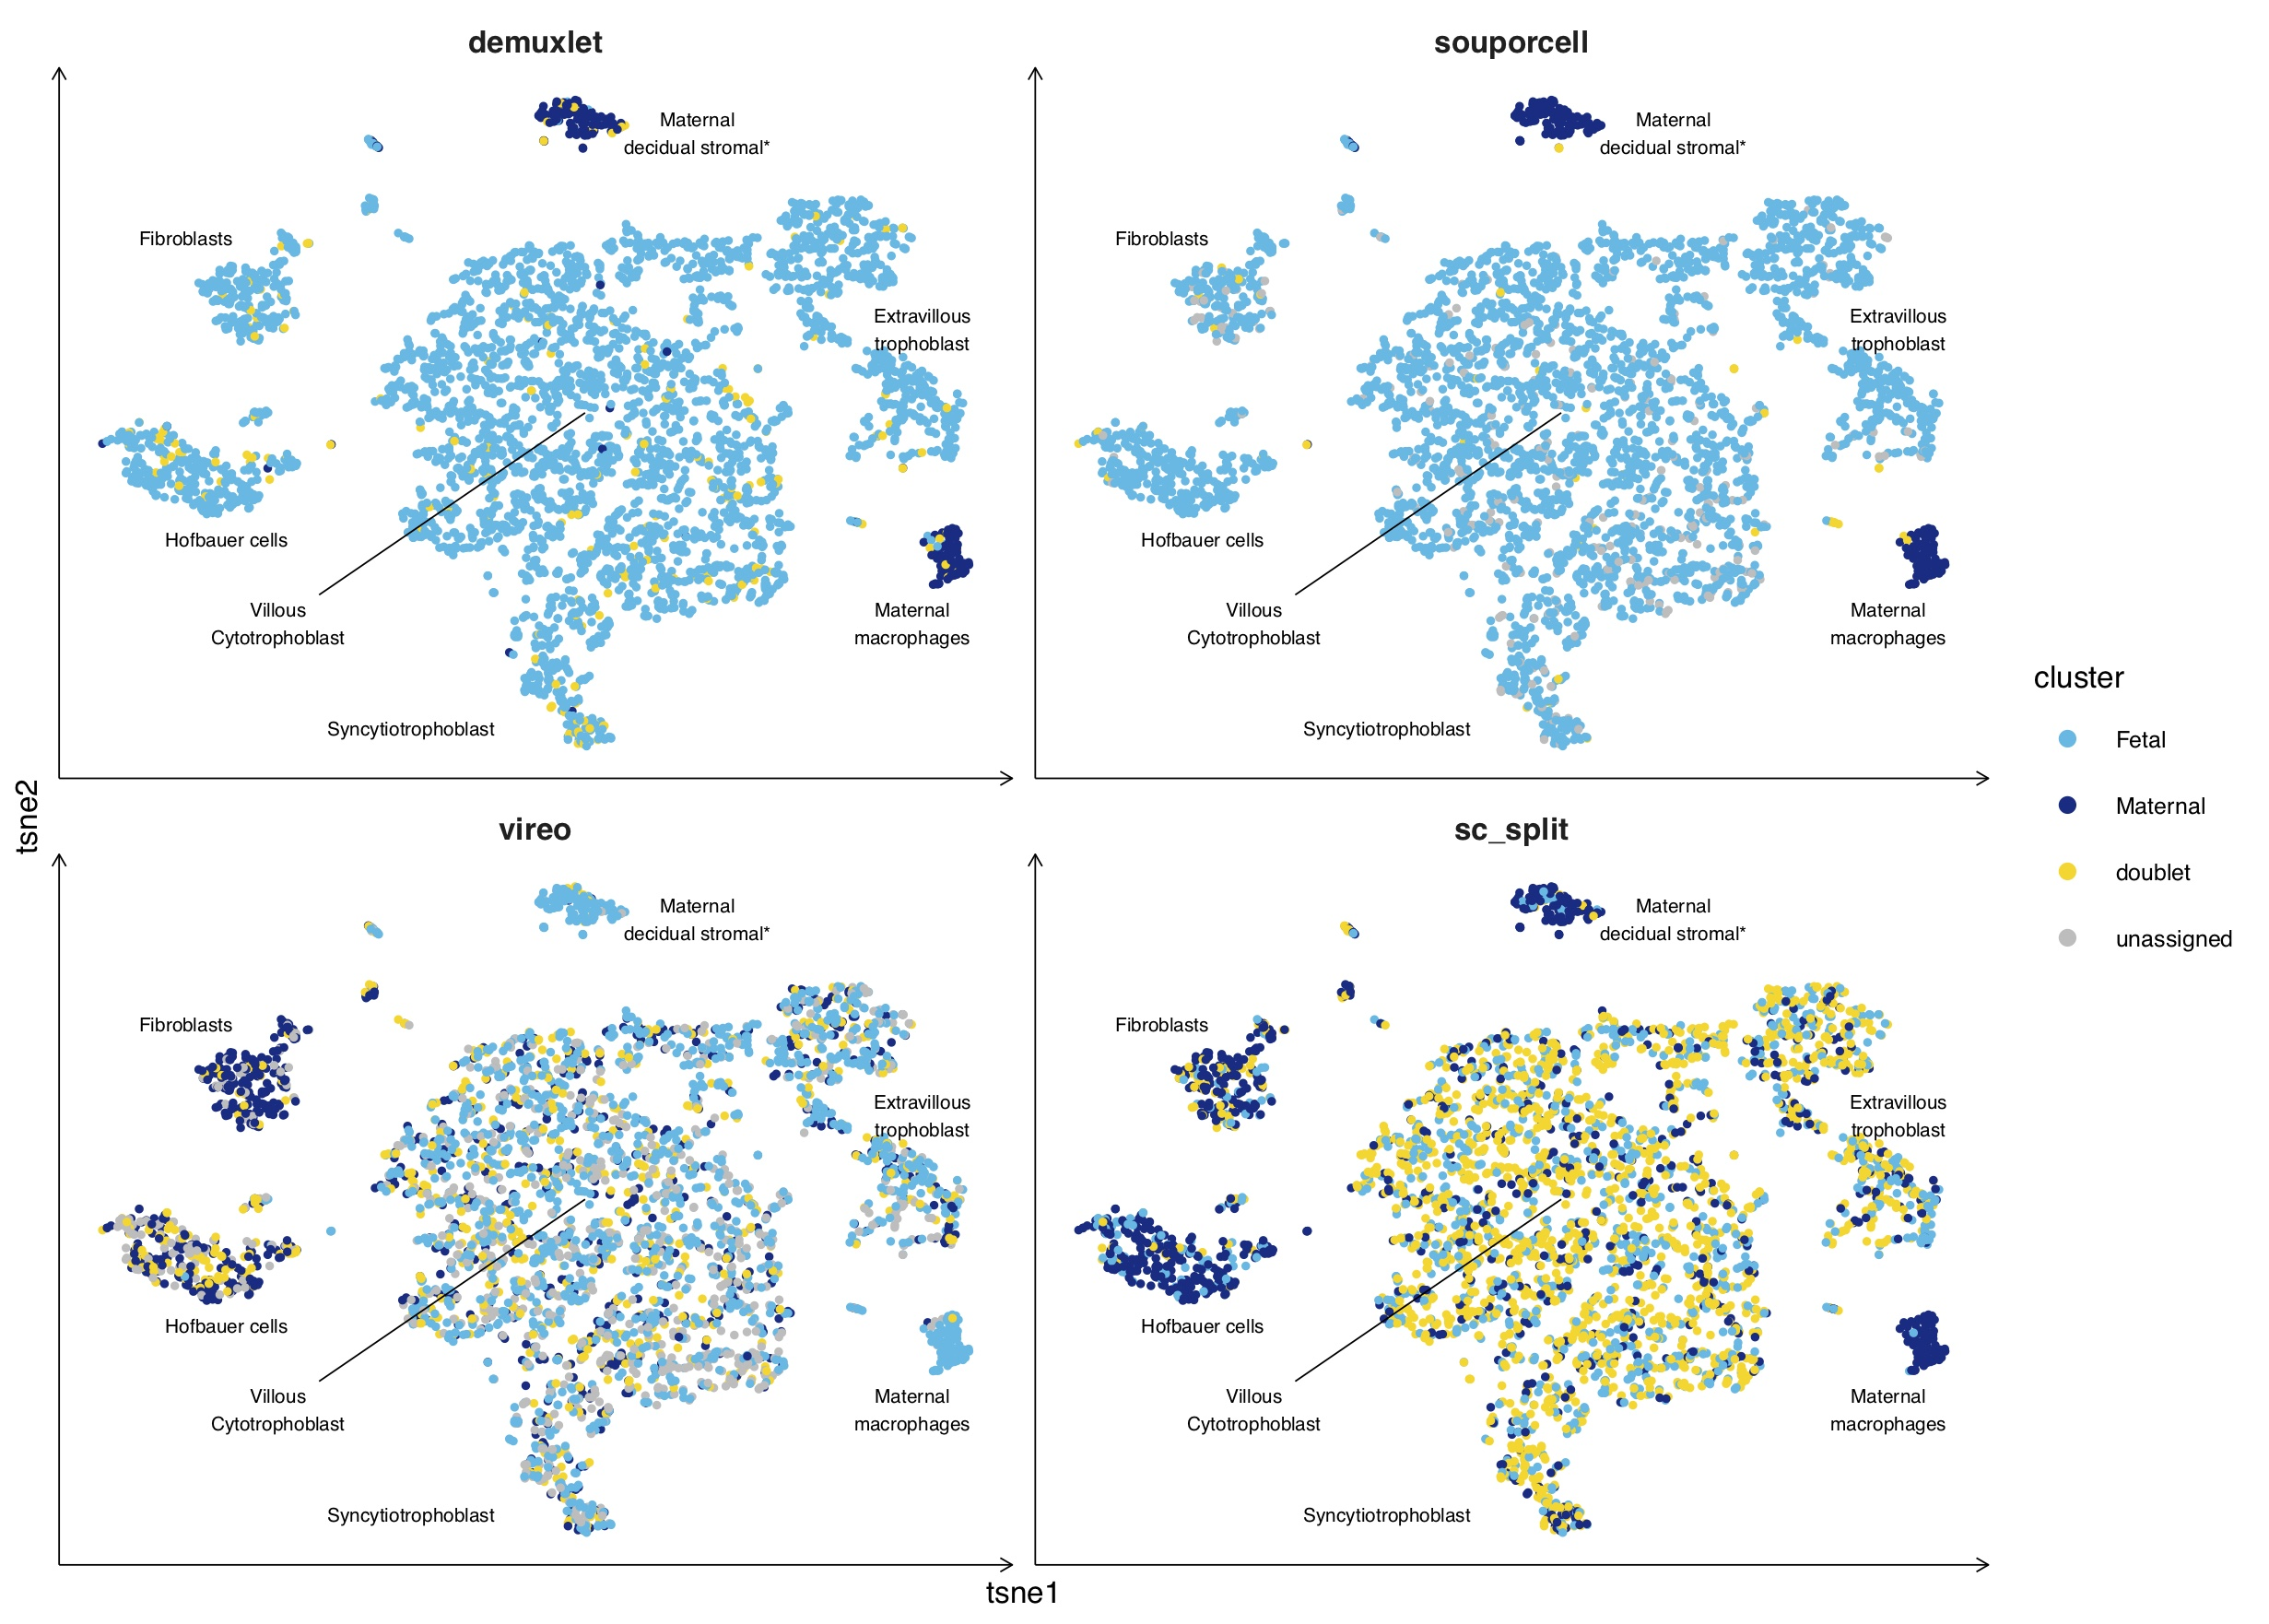
\includegraphics[width=\textwidth]{maternal.jpg} 
\par{Cell expression t-SNE plots of n=3,835 cells colored by each tool's genotype assignments or clusters for a placental sample. Cell phenotype clusters and cell genotype clusters co-segregate, with the majority of cell types being of fetal origin with the exception of maternal macrophages and *maternal decidual stromal cells, the latter of which (found only in one donor) were considered to be a non-placental artefact arising from the surgical procedure and were removed during data quality control in the original study\cite{maternalfetal}. We observe high concordance between souporcell and demuxlet (ARI 0.96) whereas vireo and scSplit have large discordances with ARI of 0 and 0.03 respectively.}

\end{centering}
\end{figure}


\subsection{Plasmodium}

\begin{figure}[htbp!]
\caption{Plasmodium data}
\label{figure:malaria}
\begin{centering}

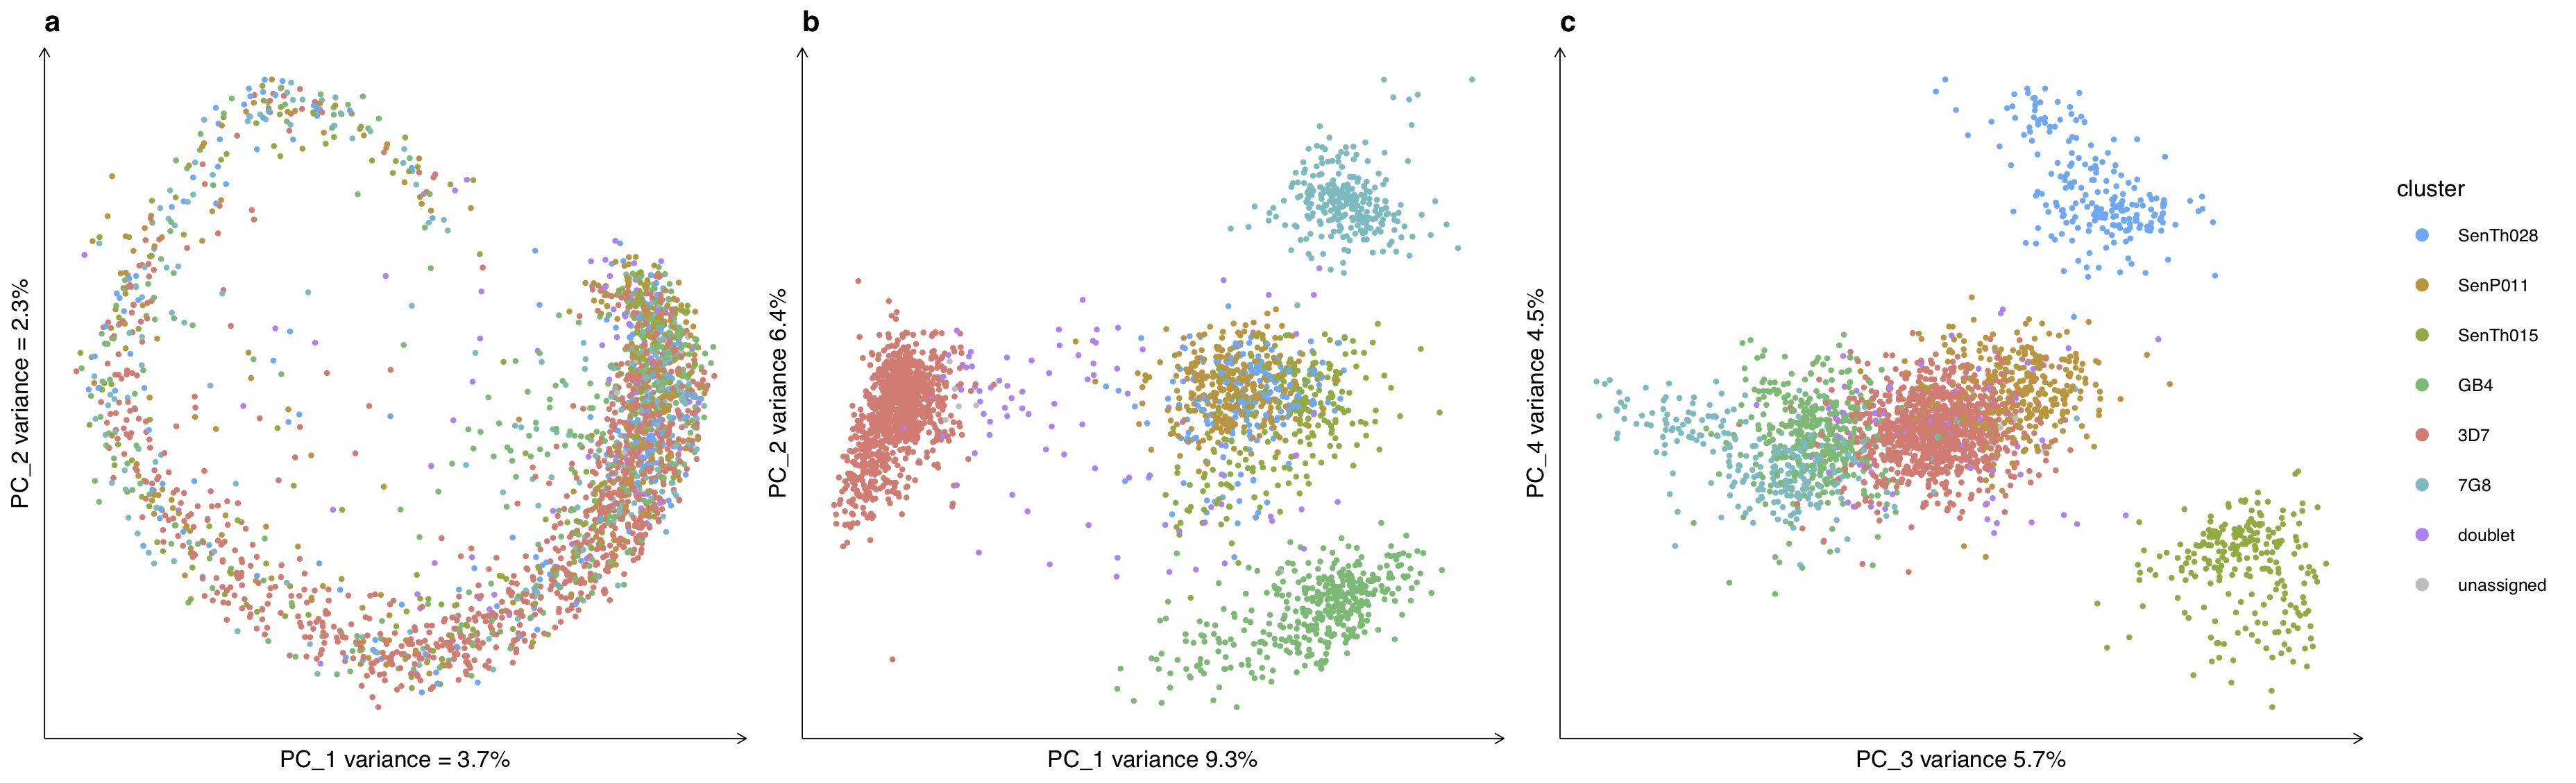
\includegraphics[width=\textwidth]{malaria.jpg} 
\par{\textbf{b)} Expression PCA colored by genotype clusters for Plasmodium sample 1 (n=2608 cells) (other samples in Fig. S3) showing an even spread of genotypes throughout the asexual lifecycle. \textbf{b} and \textbf{c)} PCAs of first four PCs of souporcell's normalized cell-by-cluster loss matrix showing good separation of each genotypic cluster (n=2608 cells).}

\end{centering}
\end{figure}

\par{
We also tested souporcell on a non-human sample, the single-celled malaria parasite \textit{Plasmodium falciparum}, for which single cell approaches are now used to explore natural infections\cite{MCA}. Malaria infections often contain parasites from multiple different genetic backgrounds, and it is not possible to separate the strains prior to sequencing. These samples differ from human samples in a variety of ways; they are haploid when infecting humans, the genome is $>80$\% A/T, and the transcriptome is only $\sim12$ megabases (genome is $\sim23$ Mb). We generated three datasets containing six genetically distinct strains of \textit{P. falciparum} (methods) sampling 1893-2608 cells with median UMIs of ~1000. Analysis of the expression profile of one of these (see Fig. S3 for the others) reveals that the genotypes are distributed across the \textit{Plasmodium} intra-erythrocytic cycle (\ref{figure:malaria}a) while being well separated in normalized loss cluster space (\ref{figure:malaria}b,c). The ARI for each method on the three \textit{Plasmodium} data sets show superior performance for souporcell across the board, with scSplit suffering on all datasets and vireo performing poorly on one, which had an ARI versus demuxlet of 0.24. This sample was more difficult due to sample skew caused by a clonal expansion of one of the six strains.
}

\par{
We did three \textit{Plasmodium falciparum} mixture experiments. In the one shown above, the cells were mixed and immediately prepared for single cell sequencing. In the second one, the cells were mixed and then fixed in methanol before being prepared for scRNAseq. In the third mixture, cells were mixed and then grown in culture for seven days prior to single cell sequencing. Because the initial mixture was not very equal, the majority strain out grew the other strains dramatically. This caused the number of cells from some of the other strains to contain very few cells and be more difficult to cluster. Figure \ref{figure:malaria_replicates} shows the results of the 2nd and 3rd mixtures. The Plasmodium 3 sample which was cultured for seven days prior to being sequenced did not cluster into six clusters well. The elbow plot seemed to support a K of 3 more than the true number of strains mixed. This shows some of the limitations of souporcell and clustering in general with highly skewed number of cells per sample.
}


\begin{figure}[htbp!]
\caption{Plasmodium data replicates}
\label{figure:malaria_replicates}
\begin{centering}

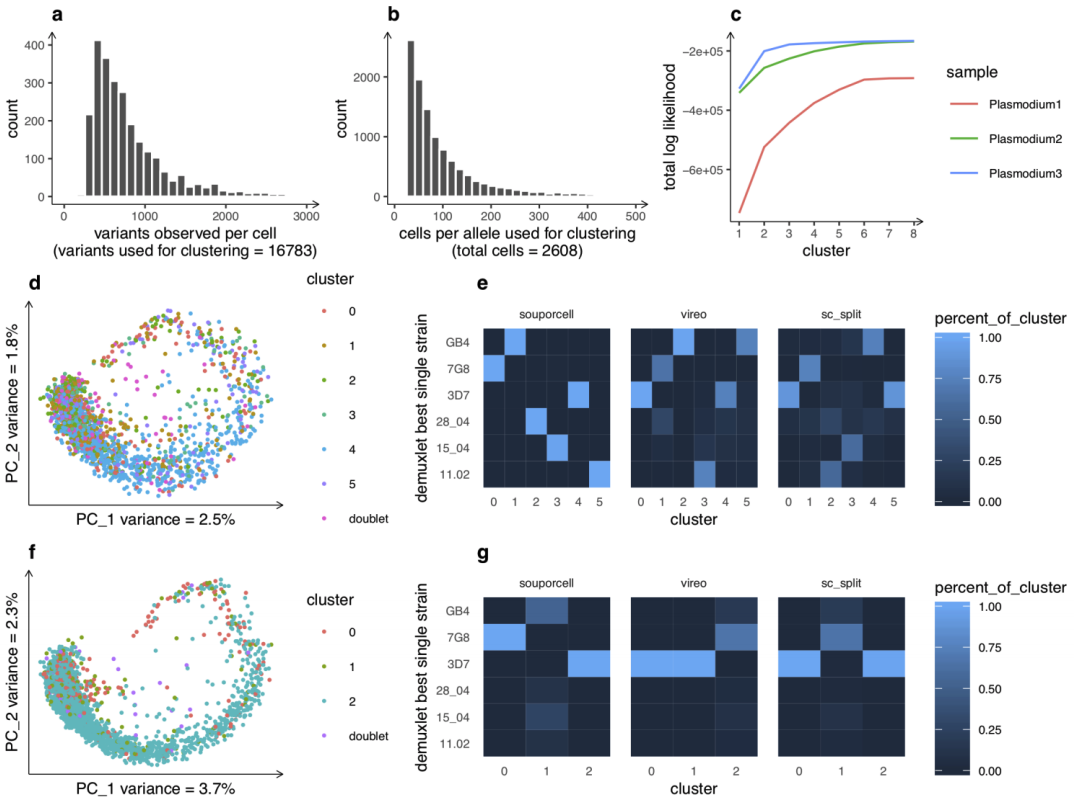
\includegraphics[width=\textwidth]{plasmodium_replicates.jpg} 
\par{\textbf{a)} Distribution of number of variants observed per cell used for clustering (with at least 4 cells required to support each allele) and the
total number of variants used for clustering on the Plasmodium1 sample. \textbf{b)} Distribution of counts of the number of cells expressing
each allele used for clustering as well as the total number of cells in the Plasmodium1 sample. \textbf{c)} Elbow plots for each Plasmodium
data set show relatively strong support for the correct number of clusters (6) for Plasmodium1, but less clear results for Plasmodium2,
which suffered from higher amounts of ambient RNA, and for Plasmodium3, which due to more cell numbers biased towards three
genotypes rather than a relatively even mixture. For this reason, we analyze Plasmodium3 with k=3. \textbf{d)} Expression PCA of the
Plasmodium2 sample (1893 cells) colored by genotype clusters as called by souporcell. \textbf{e)} Confusion matrix heatmap of the demuxlet
best single strain (Y axis) versus souporcell, vireo, and scSplit. For souporcell we see one cluster per strain as expected. Both vireo
and scSplit have the majority strain, 3D7, split across two clusters and two other strains combined into a single cluster. \textbf{f)} Expression
PCA of the Plasmodium3 sample (2293 cells) colored by genotype clusters as called by souporcell. \textbf{g}) Confusion matrix heatmap of the
demuxlet best single strain (Y axis) versus souporcell, vireo, and scSplit genotype clusters with k=3. Souporcell clusters out the 3D7
and 7G8 strains correctly and puts all other cells into the final cluster while both vireo and scSplit put 3D7 into two clusters and all other
cells into the remaining cluster.}

\end{centering}
\end{figure}




\subsection{Twenty one individual mixture demonstration}
\par{
We demonstrate that souporcell is capable of demultiplexing many donors by creating a synthetic mixture
of 21 different individuals, which given the current recommendations from 10x on cells per run would be
a high-end number of donors to multiplex. To generate this 21-donor mix, we used the 5 HipSci samples
described in \ref{figure:synthetic} and added to them 16 PBMC samples obtained from the Human Cell Atlas Census of
Immune Cells. From each dataset we randomly selected 1000 cells with at least 4000 UMIs and
simulated 10\% doublets and 2.5\% ambient RNA by altering the cell barcodes, as described above. We
clustered these with souporcell and the software correctly identifies 1690 of the 2100 synthetic doublets.
A further 69 cells were unassigned, and in total we have an ARI of 0.95. Excluding all doublets the ARI
is 0.98. We find a total of 134/16800 singletons misassigned where 129 of them are CB8 cells assigned to
the CB3 cluster. We show later that this is likely because the CB8 sample is contaminated by another
(non CB3) donor. \ref{figure:21donor} shows the UMAP projection of the normalized cluster log likelihood
matrix. It is clear that souporcell is able to handle at least 21 distinct donors and accurately assign cluster
identities to the majority of cells. 
}

\par{
Because this error type accounted for >95\% of singleton errors, we suspected this may be due to
contamination. We repeated this experiment with several of the replicates of the CB8 donor and found
consistent results. We then made a synthetic mixture of CB3 and CB8 in order to determine if this was
due to the large number of donors and it was not. We still found that roughly 20\% of CB8 cells would
cluster with CB3, but if given 3 clusters, all of those cells formed their own cluster. This made us suspect 
that the CB8 sample was contaminated with cells from a different (non CB3) donor.
}


\begin{figure}[htbp!]
\caption{21 donor example}
\label{figure:21donor}
\begin{centering}

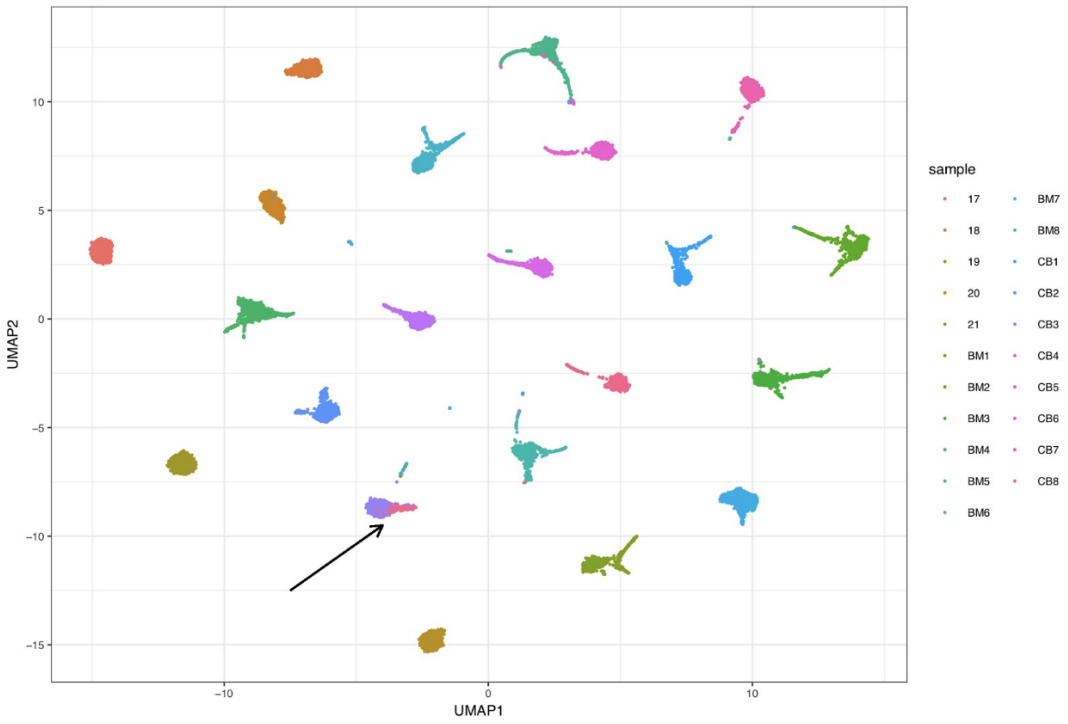
\includegraphics[width=\textwidth]{21donor.png} 
\par{Umap of the normalized log likelihood cluster matrix for the singletons of a mixture of the 5 HipSci samples and the 16 PBMC
samples from the Human Cell Atlas project. The main error is the assignment of 129 CB8 cells to the CB3 dominant cluster indi cated by
the arrow. We show later that this is likely due to contamination.}

\end{centering}
\end{figure}

\subsubsection{Contamination revealed}

To further test whether the CB8+CB3 ``misassignment" was an error or true signal, we created a synthetic mixture of all cells from both the CB8 sample and the CB3 sample. We ran souporcell with a range of k from 1 to 5 and plotted the elbow curve \ref{figure:contamination}a and the PCA of the cell cluster likelihoods for the clearly optimal number of clusters which was three. This PCA has good separation and gives good evidence that the CB8 sample was contaminated with cells from another donor which were most likely more closely related to the CB3 sample than the CB8 sample. We followed up with the creators of the census of immune cells data resource and they said that they were already aware of a contamination in the CB8 sample. This corroborated discover was not picked up by the vireo team which used the same data with which they reported high concordance. This shows further the power of souporcell for detection of unexpected events such as sample contamination.

\begin{figure}[htbp!]
\caption{Contamination revealed}
\label{figure:contamination}
\begin{centering}

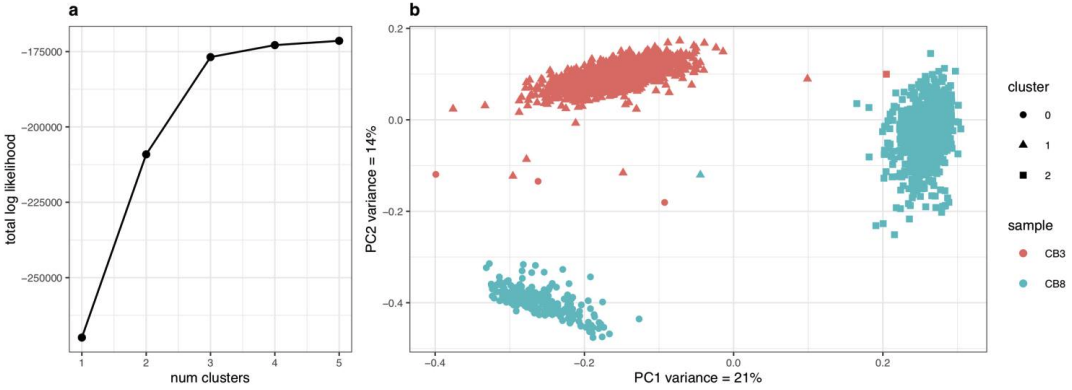
\includegraphics[width=\textwidth]{contamination.png} 
\par{\textbf{a)} Elbow plot of CB8+CB3 synthetic mixture with 3\% doublets shows a clear preference for three clusters rather than the expected two.
\textbf{b)} Shows the PCA of the normalized cell by cluster log likelihood matrix (n=2716 cells) showing three distinct genotypes.}

\end{centering}
\end{figure}

\subsubsection{Downsampling experiments for cells and UMIs}

\par{
In order to explore the regime for which it is still possible to accurately demultiplex mixed samples, we
used our synthetically mixed 5 HipSci samples and downsampled UMIs (figure \ref{figure:umidown}a) and cell (figure \ref{figure:umidown}
b) and report the ARI versus the ground truth. We find that while overall clustering remains good, cell
assignment accuracy decreases below 800 median UMI per cell and that accuracy remains high down to
an average of 40 cells per cluster (see figure \ref{figure:umidown}b). 
}

\begin{figure}[htbp!]
\caption{Performance on low UMI counts}
\label{figure:umidown}
\begin{centering}

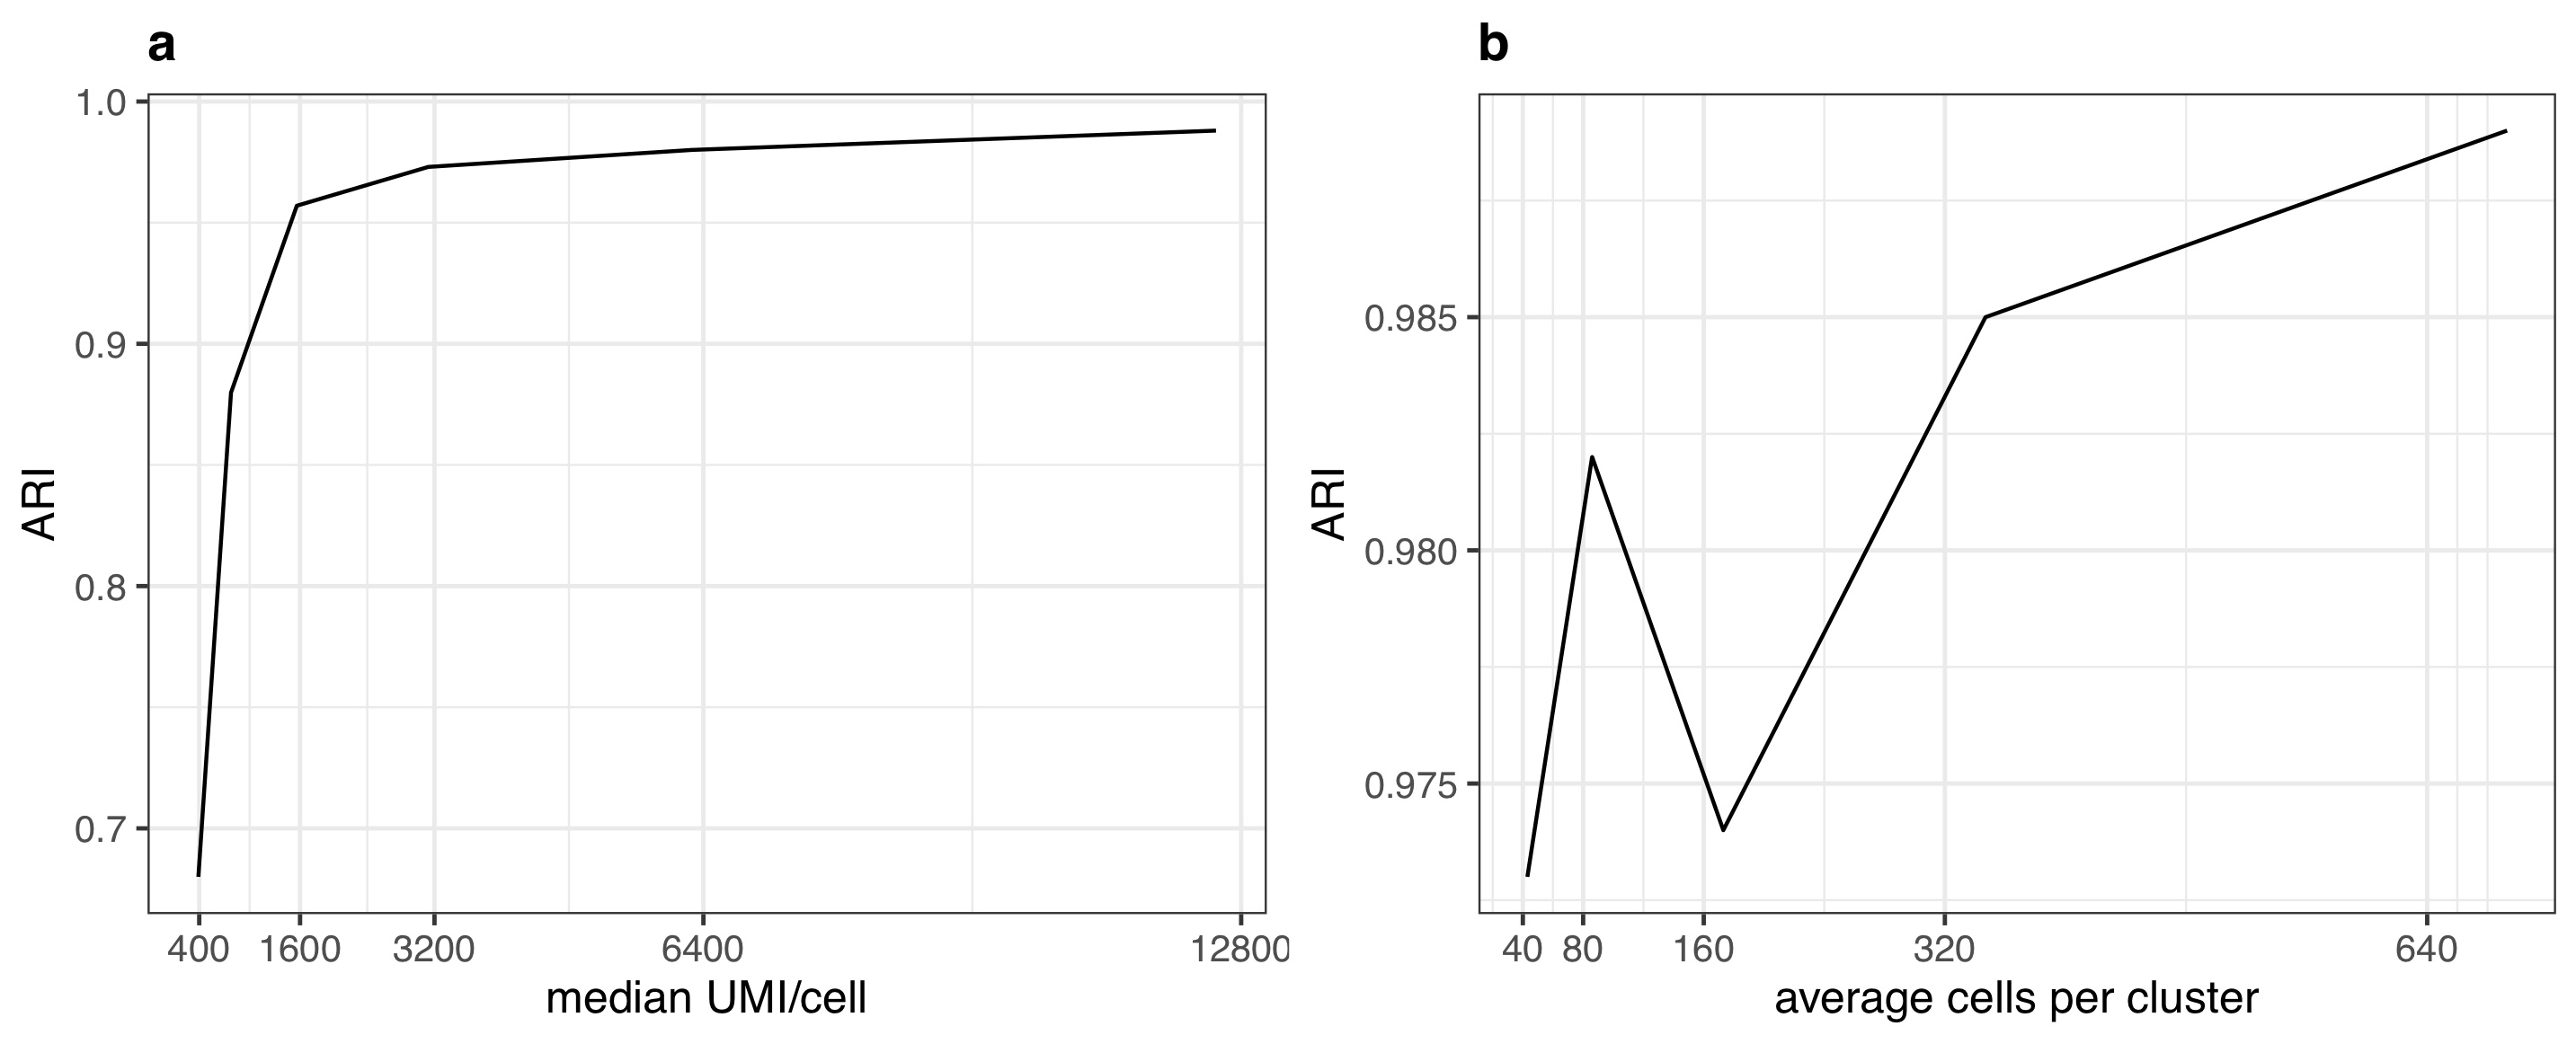
\includegraphics[width=\textwidth]{umidown.jpg} 
\par{\textbf{a)} The synthetic mixture of 5 HipSci cell lines with 6\% doublets and 5\% ambient RNA with UMIs downsampled shows predominantly
good clustering, but performance drops below 800 UMIs/cell. \textbf{b)} The clustering is consistently good with downsampled cells down to an
average cell per cluster of 40. The cluster with the fewest cells in the 40 average cells per cluster had 20 cells.}

\end{centering}
\end{figure}




\section{Discussion}
Here we have presented souporcell, a method for clustering scRNAseq cells by genotype using sparse mixture model clustering with explicit ambient RNA modeling. Our benchmarks show that souporcell can outperform all other currently available methods, including those that require genotypes a priori. Using more realistic and challenging test cases than previous studies, we show that souporcell is robust across a large range of parameters, and more so than any other currently available method. Moreover, souporcell is highly accurate for challenging datasets involving closely related maternal/fetal samples, and varying mixtures of Plasmodium falciparum strains. Limitations of souporcell include low signal to noise due to decreased UMI per cell and high numbers of donors causing increased local maxima. Due to the advantages that mixtures give to scRNAseq experiments in ameliorating batch effects, improving doublet detection, and allowing for ambient RNA estimation, souporcell enables donor multiplexing designs to be used more easily than was previously possible, including in situations when no WGS or genotyping data are available. In addition to reducing cost and allowing for more complex and robust experimental designs, souporcell also enables valuable genotype information to be extracted and ambient RNA estimation at no additional cost.

%********************************** % Third Section  *************************************

